% Options for packages loaded elsewhere
\PassOptionsToPackage{unicode}{hyperref}
\PassOptionsToPackage{hyphens}{url}
\PassOptionsToPackage{dvipsnames,svgnames,x11names}{xcolor}
%
\documentclass[
  letterpaper,
  DIV=11,
  numbers=noendperiod]{scrreprt}

\usepackage{amsmath,amssymb}
\usepackage{iftex}
\ifPDFTeX
  \usepackage[T1]{fontenc}
  \usepackage[utf8]{inputenc}
  \usepackage{textcomp} % provide euro and other symbols
\else % if luatex or xetex
  \usepackage{unicode-math}
  \defaultfontfeatures{Scale=MatchLowercase}
  \defaultfontfeatures[\rmfamily]{Ligatures=TeX,Scale=1}
\fi
\usepackage{lmodern}
\ifPDFTeX\else  
    % xetex/luatex font selection
\fi
% Use upquote if available, for straight quotes in verbatim environments
\IfFileExists{upquote.sty}{\usepackage{upquote}}{}
\IfFileExists{microtype.sty}{% use microtype if available
  \usepackage[]{microtype}
  \UseMicrotypeSet[protrusion]{basicmath} % disable protrusion for tt fonts
}{}
\makeatletter
\@ifundefined{KOMAClassName}{% if non-KOMA class
  \IfFileExists{parskip.sty}{%
    \usepackage{parskip}
  }{% else
    \setlength{\parindent}{0pt}
    \setlength{\parskip}{6pt plus 2pt minus 1pt}}
}{% if KOMA class
  \KOMAoptions{parskip=half}}
\makeatother
\usepackage{xcolor}
\setlength{\emergencystretch}{3em} % prevent overfull lines
\setcounter{secnumdepth}{5}
% Make \paragraph and \subparagraph free-standing
\ifx\paragraph\undefined\else
  \let\oldparagraph\paragraph
  \renewcommand{\paragraph}[1]{\oldparagraph{#1}\mbox{}}
\fi
\ifx\subparagraph\undefined\else
  \let\oldsubparagraph\subparagraph
  \renewcommand{\subparagraph}[1]{\oldsubparagraph{#1}\mbox{}}
\fi

\usepackage{color}
\usepackage{fancyvrb}
\newcommand{\VerbBar}{|}
\newcommand{\VERB}{\Verb[commandchars=\\\{\}]}
\DefineVerbatimEnvironment{Highlighting}{Verbatim}{commandchars=\\\{\}}
% Add ',fontsize=\small' for more characters per line
\usepackage{framed}
\definecolor{shadecolor}{RGB}{241,243,245}
\newenvironment{Shaded}{\begin{snugshade}}{\end{snugshade}}
\newcommand{\AlertTok}[1]{\textcolor[rgb]{0.68,0.00,0.00}{#1}}
\newcommand{\AnnotationTok}[1]{\textcolor[rgb]{0.37,0.37,0.37}{#1}}
\newcommand{\AttributeTok}[1]{\textcolor[rgb]{0.40,0.45,0.13}{#1}}
\newcommand{\BaseNTok}[1]{\textcolor[rgb]{0.68,0.00,0.00}{#1}}
\newcommand{\BuiltInTok}[1]{\textcolor[rgb]{0.00,0.23,0.31}{#1}}
\newcommand{\CharTok}[1]{\textcolor[rgb]{0.13,0.47,0.30}{#1}}
\newcommand{\CommentTok}[1]{\textcolor[rgb]{0.37,0.37,0.37}{#1}}
\newcommand{\CommentVarTok}[1]{\textcolor[rgb]{0.37,0.37,0.37}{\textit{#1}}}
\newcommand{\ConstantTok}[1]{\textcolor[rgb]{0.56,0.35,0.01}{#1}}
\newcommand{\ControlFlowTok}[1]{\textcolor[rgb]{0.00,0.23,0.31}{#1}}
\newcommand{\DataTypeTok}[1]{\textcolor[rgb]{0.68,0.00,0.00}{#1}}
\newcommand{\DecValTok}[1]{\textcolor[rgb]{0.68,0.00,0.00}{#1}}
\newcommand{\DocumentationTok}[1]{\textcolor[rgb]{0.37,0.37,0.37}{\textit{#1}}}
\newcommand{\ErrorTok}[1]{\textcolor[rgb]{0.68,0.00,0.00}{#1}}
\newcommand{\ExtensionTok}[1]{\textcolor[rgb]{0.00,0.23,0.31}{#1}}
\newcommand{\FloatTok}[1]{\textcolor[rgb]{0.68,0.00,0.00}{#1}}
\newcommand{\FunctionTok}[1]{\textcolor[rgb]{0.28,0.35,0.67}{#1}}
\newcommand{\ImportTok}[1]{\textcolor[rgb]{0.00,0.46,0.62}{#1}}
\newcommand{\InformationTok}[1]{\textcolor[rgb]{0.37,0.37,0.37}{#1}}
\newcommand{\KeywordTok}[1]{\textcolor[rgb]{0.00,0.23,0.31}{#1}}
\newcommand{\NormalTok}[1]{\textcolor[rgb]{0.00,0.23,0.31}{#1}}
\newcommand{\OperatorTok}[1]{\textcolor[rgb]{0.37,0.37,0.37}{#1}}
\newcommand{\OtherTok}[1]{\textcolor[rgb]{0.00,0.23,0.31}{#1}}
\newcommand{\PreprocessorTok}[1]{\textcolor[rgb]{0.68,0.00,0.00}{#1}}
\newcommand{\RegionMarkerTok}[1]{\textcolor[rgb]{0.00,0.23,0.31}{#1}}
\newcommand{\SpecialCharTok}[1]{\textcolor[rgb]{0.37,0.37,0.37}{#1}}
\newcommand{\SpecialStringTok}[1]{\textcolor[rgb]{0.13,0.47,0.30}{#1}}
\newcommand{\StringTok}[1]{\textcolor[rgb]{0.13,0.47,0.30}{#1}}
\newcommand{\VariableTok}[1]{\textcolor[rgb]{0.07,0.07,0.07}{#1}}
\newcommand{\VerbatimStringTok}[1]{\textcolor[rgb]{0.13,0.47,0.30}{#1}}
\newcommand{\WarningTok}[1]{\textcolor[rgb]{0.37,0.37,0.37}{\textit{#1}}}

\providecommand{\tightlist}{%
  \setlength{\itemsep}{0pt}\setlength{\parskip}{0pt}}\usepackage{longtable,booktabs,array}
\usepackage{calc} % for calculating minipage widths
% Correct order of tables after \paragraph or \subparagraph
\usepackage{etoolbox}
\makeatletter
\patchcmd\longtable{\par}{\if@noskipsec\mbox{}\fi\par}{}{}
\makeatother
% Allow footnotes in longtable head/foot
\IfFileExists{footnotehyper.sty}{\usepackage{footnotehyper}}{\usepackage{footnote}}
\makesavenoteenv{longtable}
\usepackage{graphicx}
\makeatletter
\def\maxwidth{\ifdim\Gin@nat@width>\linewidth\linewidth\else\Gin@nat@width\fi}
\def\maxheight{\ifdim\Gin@nat@height>\textheight\textheight\else\Gin@nat@height\fi}
\makeatother
% Scale images if necessary, so that they will not overflow the page
% margins by default, and it is still possible to overwrite the defaults
% using explicit options in \includegraphics[width, height, ...]{}
\setkeys{Gin}{width=\maxwidth,height=\maxheight,keepaspectratio}
% Set default figure placement to htbp
\makeatletter
\def\fps@figure{htbp}
\makeatother
% definitions for citeproc citations
\NewDocumentCommand\citeproctext{}{}
\NewDocumentCommand\citeproc{mm}{%
  \begingroup\def\citeproctext{#2}\cite{#1}\endgroup}
\makeatletter
 % allow citations to break across lines
 \let\@cite@ofmt\@firstofone
 % avoid brackets around text for \cite:
 \def\@biblabel#1{}
 \def\@cite#1#2{{#1\if@tempswa , #2\fi}}
\makeatother
\newlength{\cslhangindent}
\setlength{\cslhangindent}{1.5em}
\newlength{\csllabelwidth}
\setlength{\csllabelwidth}{3em}
\newenvironment{CSLReferences}[2] % #1 hanging-indent, #2 entry-spacing
 {\begin{list}{}{%
  \setlength{\itemindent}{0pt}
  \setlength{\leftmargin}{0pt}
  \setlength{\parsep}{0pt}
  % turn on hanging indent if param 1 is 1
  \ifodd #1
   \setlength{\leftmargin}{\cslhangindent}
   \setlength{\itemindent}{-1\cslhangindent}
  \fi
  % set entry spacing
  \setlength{\itemsep}{#2\baselineskip}}}
 {\end{list}}
\usepackage{calc}
\newcommand{\CSLBlock}[1]{\hfill\break\parbox[t]{\linewidth}{\strut\ignorespaces#1\strut}}
\newcommand{\CSLLeftMargin}[1]{\parbox[t]{\csllabelwidth}{\strut#1\strut}}
\newcommand{\CSLRightInline}[1]{\parbox[t]{\linewidth - \csllabelwidth}{\strut#1\strut}}
\newcommand{\CSLIndent}[1]{\hspace{\cslhangindent}#1}

\KOMAoption{captions}{tableheading}
\makeatletter
\@ifpackageloaded{bookmark}{}{\usepackage{bookmark}}
\makeatother
\makeatletter
\@ifpackageloaded{caption}{}{\usepackage{caption}}
\AtBeginDocument{%
\ifdefined\contentsname
  \renewcommand*\contentsname{Table of contents}
\else
  \newcommand\contentsname{Table of contents}
\fi
\ifdefined\listfigurename
  \renewcommand*\listfigurename{List of Figures}
\else
  \newcommand\listfigurename{List of Figures}
\fi
\ifdefined\listtablename
  \renewcommand*\listtablename{List of Tables}
\else
  \newcommand\listtablename{List of Tables}
\fi
\ifdefined\figurename
  \renewcommand*\figurename{Figure}
\else
  \newcommand\figurename{Figure}
\fi
\ifdefined\tablename
  \renewcommand*\tablename{Table}
\else
  \newcommand\tablename{Table}
\fi
}
\@ifpackageloaded{float}{}{\usepackage{float}}
\floatstyle{ruled}
\@ifundefined{c@chapter}{\newfloat{codelisting}{h}{lop}}{\newfloat{codelisting}{h}{lop}[chapter]}
\floatname{codelisting}{Listing}
\newcommand*\listoflistings{\listof{codelisting}{List of Listings}}
\makeatother
\makeatletter
\makeatother
\makeatletter
\@ifpackageloaded{caption}{}{\usepackage{caption}}
\@ifpackageloaded{subcaption}{}{\usepackage{subcaption}}
\makeatother
\ifLuaTeX
  \usepackage{selnolig}  % disable illegal ligatures
\fi
\usepackage{bookmark}

\IfFileExists{xurl.sty}{\usepackage{xurl}}{} % add URL line breaks if available
\urlstyle{same} % disable monospaced font for URLs
\hypersetup{
  pdftitle={Cookbook Data Analysis with Stata and R},
  pdfauthor={Manuel Oliveira},
  colorlinks=true,
  linkcolor={blue},
  filecolor={Maroon},
  citecolor={Blue},
  urlcolor={Blue},
  pdfcreator={LaTeX via pandoc}}

\title{Cookbook Data Analysis with Stata and R}
\author{Manuel Oliveira}
\date{2024-08-01}

\begin{document}
\maketitle

\renewcommand*\contentsname{Table of contents}
{
\hypersetup{linkcolor=}
\setcounter{tocdepth}{2}
\tableofcontents
}
\bookmarksetup{startatroot}

\chapter*{Welcome}\label{welcome}
\addcontentsline{toc}{chapter}{Welcome}

\markboth{Welcome}{Welcome}

Welcome to the ``Cookbook Data Analysis with Stata and R''! This book is
designed to be your comprehensive guide to mastering data analysis using
two of the most powerful tools available: Stata and R. Whether you are a
beginner or have some experience, this book will help you develop the
skills needed to tackle a wide range of data analysis challenges.

\section*{Why This Book?}\label{why-this-book}
\addcontentsline{toc}{section}{Why This Book?}

\markright{Why This Book?}

In the Human Technology Interaction track at TU/e, understanding and
analyzing data is crucial. This book aims to provide you with practical,
hands-on experience in data analysis, tailored specifically to the needs
of your coursework and future career. By the end of this book, you will
be able to:

\begin{itemize}
\tightlist
\item
  Import and manage data in both Stata and R.
\item
  Clean and prepare your data for analysis.
\item
  Perform a variety of statistical analyses.
\item
  Visualize your data to uncover insights.
\item
  Communicate your findings effectively.
\end{itemize}

\section*{What You Will Learn}\label{what-you-will-learn}
\addcontentsline{toc}{section}{What You Will Learn}

\markright{What You Will Learn}

Data analysis is a vast field, and this book focuses on giving you a
solid foundation in the most essential tools and techniques. Here's what
you can expect to learn:

\begin{enumerate}
\def\labelenumi{\arabic{enumi}.}
\tightlist
\item
  \textbf{Data Import and Management}: Learn how to import data from
  various sources and manage it efficiently in Stata and R.
\item
  \textbf{Data Cleaning and Preparation}: Understand the importance of
  tidy data and how to clean and prepare your datasets for analysis.
\item
  \textbf{Statistical Analysis}: Perform descriptive and inferential
  statistics to draw meaningful conclusions from your data.
\item
  \textbf{Data Visualization}: Create compelling visualizations to
  explore and present your data.
\item
  \textbf{Reproducible Research}: Learn best practices for ensuring your
  analyses are reproducible and transparent.
\end{enumerate}

\section*{Real-World Applications}\label{real-world-applications}
\addcontentsline{toc}{section}{Real-World Applications}

\markright{Real-World Applications}

Throughout this book, you will work on simulated dataset aiming to
reflect real-world examples and case studies relevant to Human
Technology Interaction. These examples will help you see how the
techniques you learn can be applied to actual research and industry
scenarios. Whether you are analyzing user behavior, evaluating the
effectiveness of a new technology, or exploring human-computer
interaction, this book will provide you with the tools you need.

\section*{Getting Started}\label{getting-started}
\addcontentsline{toc}{section}{Getting Started}

\markright{Getting Started}

To get the most out of this book, you will need to have Stata and R
installed on your computer. We recommend using the latest versions of
both software packages. Additionally, familiarity with basic statistical
concepts will be helpful, but not required, as we will cover the
necessary background along the way.

\bookmarksetup{startatroot}

\chapter{Introduction to R and Stata}\label{introduction-to-r-and-stata}

\bookmarksetup{startatroot}

\chapter{Brief History of R and
Stata}\label{brief-history-of-r-and-stata}

\section{History of R}\label{history-of-r}

R is a programming language and free software environment for
statistical computing and graphics. It was created by Ross Ihaka and
Robert Gentleman at the University of Auckland, New Zealand, and the
first public announcement of R was made in
1993{[}\textsuperscript{1}{]}{[}3{]}. The language was inspired by the S
language, which was developed at Bell Laboratories. R has since become a
popular tool among statisticians and data scientists due to its
extensive package ecosystem and active user community.

\section{History of Stata}\label{history-of-stata}

Stata is a general-purpose statistical software package created in the
mid-1980s by William Gould, a UCLA graduate, and Sean
Becketti{[}\textsuperscript{2}{]}{[}1{]}. Initially developed within the
Computing Resource Center (CRC) in Santa Monica, California, Stata was
designed to provide a powerful yet user-friendly environment for data
analysis. The first version of Stata was released in 1985, and it has
since evolved to include a wide range of statistical, graphical, and
data management capabilities.

\section{Comparison of R and Stata}\label{comparison-of-r-and-stata}

\begin{longtable}[]{@{}
  >{\raggedright\arraybackslash}p{(\columnwidth - 4\tabcolsep) * \real{0.1509}}
  >{\raggedright\arraybackslash}p{(\columnwidth - 4\tabcolsep) * \real{0.4214}}
  >{\raggedright\arraybackslash}p{(\columnwidth - 4\tabcolsep) * \real{0.4277}}@{}}
\toprule\noalign{}
\begin{minipage}[b]{\linewidth}\raggedright
Feature
\end{minipage} & \begin{minipage}[b]{\linewidth}\raggedright
R
\end{minipage} & \begin{minipage}[b]{\linewidth}\raggedright
Stata
\end{minipage} \\
\midrule\noalign{}
\endhead
\bottomrule\noalign{}
\endlastfoot
\textbf{Cost} & Free and open-source & Paid software \\
\textbf{User Interface} & Command-line interface, with various IDEs like
RStudio available & User-friendly GUI and command-line interface \\
\textbf{Flexibility} & Highly flexible, suitable for custom analyses and
new methods & Less flexible, but highly efficient for standard
statistical tasks \\
\textbf{Packages} & Extensive package ecosystem for various analyses and
visualizations & Comprehensive built-in functions and user-written
commands \\
\textbf{Learning Curve} & Steeper learning curve, especially for
beginners & Easier to learn, with simpler syntax \\
\textbf{Community Support} & Large, active community with extensive
online resources & Smaller community, but excellent official
documentation \\
\textbf{Reproducibility} & Strong support for reproducible research
through RMarkdown and other tools & Good support for reproducibility,
but less integrated than R \\
\textbf{Data Management} & Powerful data manipulation capabilities with
packages like dplyr & Efficient data manipulation and management
built-in \\
\textbf{Visualization} & Advanced visualization capabilities with
ggplot2 and other packages & Good visualization tools, but less flexible
than R \\
\end{longtable}

{[}\textsuperscript{2}{]}{[}1{]}: A brief history of Stata on its 20th
anniversary. The Stata Journal (2005). {[}\textsuperscript{1}{]}{[}3{]}:
History and Overview of R. R Programming for Data Science - Bookdown.

\bookmarksetup{startatroot}

\chapter{Chapter 1: Getting Started}\label{chapter-1-getting-started}

\section{Introduction}\label{introduction}

This chapter provides a quick tutorial on how to install and set up R
and Stata on both Windows and Mac computers. By the end of this chapter,
you'll have the necessary tools ready to begin your analysis.

\section{Installing R}\label{installing-r}

\subsection{Windows}\label{windows}

\begin{enumerate}
\def\labelenumi{\arabic{enumi}.}
\tightlist
\item
  \textbf{Download R}:

  \begin{itemize}
  \tightlist
  \item
    Go to the \href{https://cran.r-project.org/}{R Project website}.
  \item
    Click on ``Download R for Windows.''
  \item
    Click on ``base'' to download the base R package.
  \end{itemize}
\item
  \textbf{Install R}:

  \begin{itemize}
  \tightlist
  \item
    Run the downloaded \texttt{.exe} file.
  \item
    Follow the installation instructions, accepting the default
    settings.
  \end{itemize}
\item
  \textbf{Install RStudio} (Optional but recommended):

  \begin{itemize}
  \tightlist
  \item
    Download RStudio from the
    \href{https://rstudio.com/products/rstudio/download/}{RStudio
    website}.
  \item
    Run the installer and follow the setup instructions.
  \end{itemize}
\end{enumerate}

\subsection{Mac}\label{mac}

\begin{enumerate}
\def\labelenumi{\arabic{enumi}.}
\tightlist
\item
  \textbf{Download R}:

  \begin{itemize}
  \tightlist
  \item
    Visit the \href{https://cran.r-project.org/}{R Project website}.
  \item
    Click on ``Download R for macOS.''
  \end{itemize}
\item
  \textbf{Install R}:

  \begin{itemize}
  \tightlist
  \item
    Open the downloaded \texttt{.pkg} file.
  \item
    Follow the installation instructions.
  \end{itemize}
\item
  \textbf{Install RStudio} (Optional but recommended):

  \begin{itemize}
  \tightlist
  \item
    Download RStudio from the
    \href{https://rstudio.com/products/rstudio/download/}{RStudio
    website}.
  \item
    Open the \texttt{.dmg} file and drag RStudio to your Applications
    folder.
  \end{itemize}
\end{enumerate}

\section{Installing Stata}\label{installing-stata}

\subsection{Windows}\label{windows-1}

\begin{enumerate}
\def\labelenumi{\arabic{enumi}.}
\tightlist
\item
  \textbf{Obtain a License}:

  \begin{itemize}
  \tightlist
  \item
    Stata is commercial software. Ensure you have a valid license.
  \end{itemize}
\item
  \textbf{Download Stata}:

  \begin{itemize}
  \tightlist
  \item
    Go to the \href{https://www.stata.com/}{Stata website} and log in to
    your account to download the installer.
  \end{itemize}
\item
  \textbf{Install Stata}:

  \begin{itemize}
  \tightlist
  \item
    Run the downloaded \texttt{.exe} file.
  \item
    Follow the installation instructions, entering your license
    information when prompted.
  \end{itemize}
\end{enumerate}

\subsection{Mac}\label{mac-1}

\begin{enumerate}
\def\labelenumi{\arabic{enumi}.}
\tightlist
\item
  \textbf{Obtain a License}:

  \begin{itemize}
  \tightlist
  \item
    Make sure you have a valid license for Stata.
  \end{itemize}
\item
  \textbf{Download Stata}:

  \begin{itemize}
  \tightlist
  \item
    Visit the \href{https://www.stata.com/}{Stata website} and log in to
    your account to download the installer.
  \end{itemize}
\item
  \textbf{Install Stata}:

  \begin{itemize}
  \tightlist
  \item
    Open the downloaded \texttt{.dmg} file.
  \item
    Drag the Stata application to your Applications folder.
  \item
    Launch Stata and enter your license information.
  \end{itemize}
\end{enumerate}

\section{Setting Up Your Environment}\label{setting-up-your-environment}

\subsection{R Setup}\label{r-setup}

\begin{enumerate}
\def\labelenumi{\arabic{enumi}.}
\tightlist
\item
  \textbf{Open RStudio} (or R GUI if not using RStudio).
\item
  \textbf{Install Essential Packages}:

  \begin{itemize}
  \tightlist
  \item
    Open the Console and run:
  \end{itemize}
\end{enumerate}

\begin{Shaded}
\begin{Highlighting}[]
   \FunctionTok{install.packages}\NormalTok{(}\FunctionTok{c}\NormalTok{(}\StringTok{"tidyverse"}\NormalTok{, }\StringTok{"lme4"}\NormalTok{, }\StringTok{"ggplot2"}\NormalTok{))}
\end{Highlighting}
\end{Shaded}

\begin{enumerate}
\def\labelenumi{\arabic{enumi}.}
\setcounter{enumi}{2}
\tightlist
\item
  \textbf{Create a New Project} (Optional but recommended in RStudio):

  \begin{itemize}
  \tightlist
  \item
    Go to ``File'' \textgreater{} ``New Project'' \textgreater{} ``New
    Directory'' \textgreater{} ``New Project.''
  \item
    Choose a location and name for your project, then click ``Create
    Project.''
  \end{itemize}
\end{enumerate}

\subsection{Stata Setup}\label{stata-setup}

\begin{enumerate}
\def\labelenumi{\arabic{enumi}.}
\tightlist
\item
  \textbf{Open Stata}.
\item
  \textbf{Set a Working Directory}:

  \begin{itemize}
  \tightlist
  \item
    Use the command:
  \end{itemize}
\end{enumerate}

\begin{Shaded}
\begin{Highlighting}[]
\NormalTok{   cd }\StringTok{"path/to/your/directory"}
\end{Highlighting}
\end{Shaded}

Replace \texttt{"path/to/your/directory"} with the path where you want
to save your files.

\begin{enumerate}
\def\labelenumi{\arabic{enumi}.}
\setcounter{enumi}{2}
\tightlist
\item
  \textbf{Creating Do-Files}:

  \begin{itemize}
  \tightlist
  \item
    Go to ``File'' \textgreater{} ``New Do-file Editor.''
  \item
    Save the Do-file in your working directory.
  \end{itemize}
\end{enumerate}

\section{Verification}\label{verification}

\subsection{R}\label{r}

\begin{enumerate}
\def\labelenumi{\arabic{enumi}.}
\tightlist
\item
  \textbf{Test Installation}:

  \begin{itemize}
  \tightlist
  \item
    In RStudio or R GUI, type:
  \end{itemize}
\end{enumerate}

\begin{Shaded}
\begin{Highlighting}[]
   \FunctionTok{print}\NormalTok{(}\StringTok{"R is working!"}\NormalTok{)}
\end{Highlighting}
\end{Shaded}

\begin{itemize}
\tightlist
\item
  If you see the output \texttt{{[}1{]}\ "R\ is\ working!"}, your
  installation is successful.
\end{itemize}

\begin{enumerate}
\def\labelenumi{\arabic{enumi}.}
\setcounter{enumi}{1}
\tightlist
\item
  \textbf{Load a Package}:

  \begin{itemize}
  \tightlist
  \item
    Run:
  \end{itemize}
\end{enumerate}

\begin{Shaded}
\begin{Highlighting}[]
   \FunctionTok{library}\NormalTok{(ggplot2)}
   \FunctionTok{print}\NormalTok{(}\StringTok{"ggplot2 is loaded!"}\NormalTok{)}
\end{Highlighting}
\end{Shaded}

\subsection{Stata}\label{stata}

\begin{enumerate}
\def\labelenumi{\arabic{enumi}.}
\tightlist
\item
  \textbf{Test Installation}:

  \begin{itemize}
  \tightlist
  \item
    In the Command window, type:
  \end{itemize}
\end{enumerate}

\begin{Shaded}
\begin{Highlighting}[]
   \KeywordTok{display} \StringTok{"Stata is working!"}
\end{Highlighting}
\end{Shaded}

\begin{itemize}
\tightlist
\item
  If you see the output \texttt{Stata\ is\ working!}, your installation
  is successful.
\end{itemize}

\begin{enumerate}
\def\labelenumi{\arabic{enumi}.}
\setcounter{enumi}{1}
\tightlist
\item
  \textbf{Check Version}:

  \begin{itemize}
  \tightlist
  \item
    Type:
  \end{itemize}
\end{enumerate}

\begin{Shaded}
\begin{Highlighting}[]
\NormalTok{   about}
\end{Highlighting}
\end{Shaded}

\begin{itemize}
\tightlist
\item
  This will display the version of Stata installed.
\end{itemize}

\begin{center}\rule{0.5\linewidth}{0.5pt}\end{center}

With your environment set up, you're now ready to start performing
analyses using R and Stata!

\bookmarksetup{startatroot}

\chapter{t-test}\label{t-test}

\section{Brief Explanation}\label{brief-explanation}

The t-test, proposed by William Sealy Gosset under the pseudonym
``Student'' in 1908, is used to determine if there is a significant
difference between the means of two groups. It is commonly used when the
sample sizes are small and the population variance is unknown.

\begin{longtable}[]{@{}
  >{\raggedright\arraybackslash}p{(\columnwidth - 2\tabcolsep) * \real{0.4444}}
  >{\raggedright\arraybackslash}p{(\columnwidth - 2\tabcolsep) * \real{0.5556}}@{}}
\toprule\noalign{}
\begin{minipage}[b]{\linewidth}\raggedright
Statistic
\end{minipage} & \begin{minipage}[b]{\linewidth}\raggedright
Description
\end{minipage} \\
\midrule\noalign{}
\endhead
\bottomrule\noalign{}
\endlastfoot
\textbf{Proposed by} & William Sealy Gosset (1908) \\
\textbf{Purpose} & Compare means of two groups \\
\textbf{When to use} & Small sample sizes, unknown population
variance \\
\textbf{Example question} & Is there a significant difference in user
satisfaction between two versions of a software? \\
\textbf{Analytical goal} & Determine if the mean satisfaction scores
differ significantly between the two versions \\
\end{longtable}

\section{Research Question and
Hypothesis}\label{research-question-and-hypothesis}

In today's fast-paced digital world, user experience (UX) is a critical
factor that can make or break a product. Imagine a tech company,
``InnovateTech,'' which has recently launched a new interface design for
its flagship software. The company is keen to understand whether this
new design truly enhances user satisfaction compared to the old design.

InnovateTech has invested significant resources into redesigning its
software interface, aiming to make it more intuitive, visually
appealing, and user-friendly. The old design, while functional, received
mixed reviews from users, with common complaints about its complexity
and outdated look. The new design promises a sleek, modern interface
with improved navigation and enhanced features.

To validate the effectiveness of the new design, InnovateTech conducts a
study involving a diverse group of users. Participants are randomly
assigned to use either the old or the new interface for a week. At the
end of the week, they complete a detailed satisfaction survey. The
company hopes that the results will provide clear insights into whether
the new design meets user expectations and enhances their overall
experience.

\textbf{Research Question:} Does the new interface design improve user
satisfaction compared to the old design?

\textbf{Hypothesis:} Users will report higher satisfaction scores with
the new interface design compared to the old design.

\section{R packages}\label{r-packages}

\begin{Shaded}
\begin{Highlighting}[]
\CommentTok{\# Load the necessary packages }
\FunctionTok{library}\NormalTok{(tidyverse) }\CommentTok{\# used for data manipulation and visualization}
\end{Highlighting}
\end{Shaded}

\begin{verbatim}
-- Attaching core tidyverse packages ------------------------ tidyverse 2.0.0 --
v dplyr     1.1.4     v readr     2.1.5
v forcats   1.0.0     v stringr   1.5.1
v ggplot2   3.5.0     v tibble    3.2.1
v lubridate 1.9.3     v tidyr     1.3.1
v purrr     1.0.2     
-- Conflicts ------------------------------------------ tidyverse_conflicts() --
x dplyr::filter() masks stats::filter()
x dplyr::lag()    masks stats::lag()
i Use the conflicted package (<http://conflicted.r-lib.org/>) to force all conflicts to become errors
\end{verbatim}

\begin{Shaded}
\begin{Highlighting}[]
\FunctionTok{library}\NormalTok{(ggrain) }\CommentTok{\# used for raincloud plots}
\end{Highlighting}
\end{Shaded}

\begin{verbatim}
Registered S3 methods overwritten by 'ggpp':
  method                  from   
  heightDetails.titleGrob ggplot2
  widthDetails.titleGrob  ggplot2
\end{verbatim}

\begin{Shaded}
\begin{Highlighting}[]
\FunctionTok{library}\NormalTok{(cowplot) }\CommentTok{\# for cowplot theme in ggplot}
\end{Highlighting}
\end{Shaded}

\begin{verbatim}

Attaching package: 'cowplot'

The following object is masked from 'package:lubridate':

    stamp
\end{verbatim}

\begin{Shaded}
\begin{Highlighting}[]
\FunctionTok{library}\NormalTok{(Statamarkdown) }\CommentTok{\# to run Stata commands in an R environment}
\end{Highlighting}
\end{Shaded}

\begin{verbatim}
Stata found at C:/Program Files/Stata18/StataBE-64.exe
The 'stata' engine is ready to use.
\end{verbatim}

\begin{Shaded}
\begin{Highlighting}[]
\CommentTok{\# Statamarkdown configuration}
\NormalTok{stataexe }\OtherTok{\textless{}{-}} \StringTok{"C:/Program Files/Stata18/StataBE{-}64.exe"} \CommentTok{\# Add your own path to the Stata executable here if you want to try this out}
\NormalTok{knitr}\SpecialCharTok{::}\NormalTok{opts\_chunk}\SpecialCharTok{$}\FunctionTok{set}\NormalTok{(}\AttributeTok{engine.path=}\FunctionTok{list}\NormalTok{(}\AttributeTok{stata=}\NormalTok{stataexe))}

\CommentTok{\# to install any missing packages go to the Terminal and run the command: install.packages("PACKAGE\_NAME")}
\end{Highlighting}
\end{Shaded}

\section{Simulated Dataset}\label{simulated-dataset}

\subsection{In R}\label{in-r}

\begin{Shaded}
\begin{Highlighting}[]
\FunctionTok{set.seed}\NormalTok{(}\DecValTok{123}\NormalTok{)}
\NormalTok{n }\OtherTok{\textless{}{-}} \DecValTok{30}
\NormalTok{old\_design }\OtherTok{\textless{}{-}} \FunctionTok{rnorm}\NormalTok{(n, }\AttributeTok{mean =} \DecValTok{70}\NormalTok{, }\AttributeTok{sd =} \DecValTok{10}\NormalTok{)}
\NormalTok{new\_design }\OtherTok{\textless{}{-}} \FunctionTok{rnorm}\NormalTok{(n, }\AttributeTok{mean =} \DecValTok{75}\NormalTok{, }\AttributeTok{sd =} \DecValTok{10}\NormalTok{)}
\NormalTok{data }\OtherTok{\textless{}{-}} \FunctionTok{data.frame}\NormalTok{(}
  \AttributeTok{group =} \FunctionTok{rep}\NormalTok{(}\FunctionTok{c}\NormalTok{(}\StringTok{"Old Design"}\NormalTok{, }\StringTok{"New Design"}\NormalTok{), }\AttributeTok{each =}\NormalTok{ n),}
  \AttributeTok{satisfaction =} \FunctionTok{c}\NormalTok{(old\_design, new\_design)}
\NormalTok{)}
\FunctionTok{write.csv}\NormalTok{(data, }\StringTok{"satisfaction\_data.csv"}\NormalTok{, }\AttributeTok{row.names =} \ConstantTok{FALSE}\NormalTok{)}
\end{Highlighting}
\end{Shaded}

\subsection{In Stata}\label{in-stata}

\begin{Shaded}
\begin{Highlighting}[]
\KeywordTok{clear}
\KeywordTok{set} \DecValTok{seed}\NormalTok{ 123}
\KeywordTok{set} \KeywordTok{obs}\NormalTok{ 30}
\KeywordTok{gen} \FunctionTok{group}\NormalTok{ = }\StringTok{"Old Design"}
\KeywordTok{gen}\NormalTok{ satisfaction = rnormal(70, 10)}
\KeywordTok{save}\NormalTok{ old\_design.dta, }\KeywordTok{replace}
\end{Highlighting}
\end{Shaded}

\begin{verbatim}
Number of observations (_N) was 0, now 30.



file old_design.dta saved
\end{verbatim}

\begin{Shaded}
\begin{Highlighting}[]
\KeywordTok{clear}
\KeywordTok{set} \KeywordTok{obs}\NormalTok{ 30}
\KeywordTok{gen} \FunctionTok{group}\NormalTok{ = }\StringTok{"New Design"}
\KeywordTok{gen}\NormalTok{ satisfaction = rnormal(75, 10)}
\KeywordTok{save}\NormalTok{ new\_design.dta, }\KeywordTok{replace}
\end{Highlighting}
\end{Shaded}

\begin{verbatim}
Number of observations (_N) was 0, now 30.



file new_design.dta saved
\end{verbatim}

\begin{Shaded}
\begin{Highlighting}[]
\KeywordTok{use}\NormalTok{ old\_design.dta}
\KeywordTok{append} \KeywordTok{using}\NormalTok{ new\_design.dta}
\KeywordTok{save}\NormalTok{ satisfaction\_data.dta, }\KeywordTok{replace}
\end{Highlighting}
\end{Shaded}

\begin{verbatim}
file satisfaction_data.dta saved
\end{verbatim}

\section{Statistical Analysis}\label{statistical-analysis}

\subsection{Inspecting Data Descriptives and
Plotting}\label{inspecting-data-descriptives-and-plotting}

\subsubsection{In Stata}\label{in-stata-1}

\begin{Shaded}
\begin{Highlighting}[]
\KeywordTok{use}\NormalTok{ satisfaction\_data.dta}
\KeywordTok{summarize}\NormalTok{ satisfaction}
\KeywordTok{graph}\NormalTok{ box satisfaction, }\BaseNTok{over}\NormalTok{(}\FunctionTok{group}\NormalTok{)}
\end{Highlighting}
\end{Shaded}

\begin{verbatim}
    Variable |        Obs        Mean    Std. dev.       Min        Max
-------------+---------------------------------------------------------
satisfaction |         60    72.69432    11.03765   50.47923   99.36316
\end{verbatim}

\subsubsection{In R}\label{in-r-1}

\begin{Shaded}
\begin{Highlighting}[]
\NormalTok{data }\OtherTok{\textless{}{-}} \FunctionTok{read.csv}\NormalTok{(}\StringTok{"satisfaction\_data.csv"}\NormalTok{)}
\FunctionTok{summary}\NormalTok{(data}\SpecialCharTok{$}\NormalTok{satisfaction)}
\end{Highlighting}
\end{Shaded}

\begin{verbatim}
   Min. 1st Qu.  Median    Mean 3rd Qu.    Max. 
  50.33   65.48   73.26   73.16   80.62   96.69 
\end{verbatim}

\begin{Shaded}
\begin{Highlighting}[]
\NormalTok{p }\OtherTok{\textless{}{-}} \FunctionTok{ggplot}\NormalTok{(data, }\FunctionTok{aes}\NormalTok{(}\AttributeTok{x =}\NormalTok{ group, }\AttributeTok{y =}\NormalTok{ satisfaction)) }\SpecialCharTok{+}
  \FunctionTok{geom\_boxplot}\NormalTok{() }\SpecialCharTok{+}
  \FunctionTok{theme\_cowplot}\NormalTok{() }\SpecialCharTok{+}
  \FunctionTok{labs}\NormalTok{(}\AttributeTok{title =} \StringTok{"Satisfaction Scores by Group"}\NormalTok{, }\AttributeTok{x =} \StringTok{"Group"}\NormalTok{, }\AttributeTok{y =} \StringTok{"Satisfaction Score"}\NormalTok{)}
\NormalTok{p}
\end{Highlighting}
\end{Shaded}

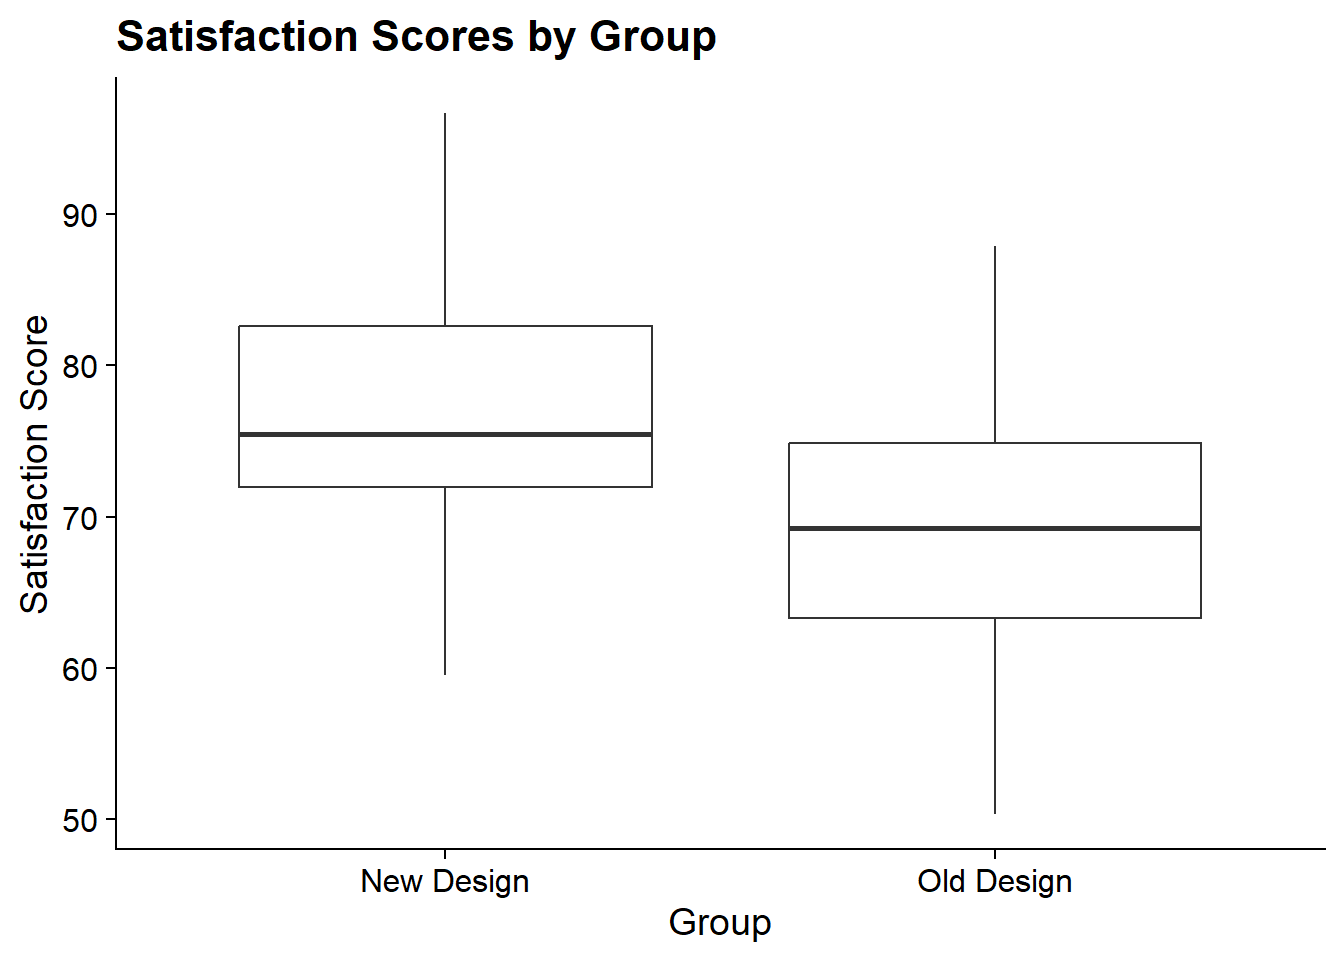
\includegraphics{ttest_files/figure-pdf/unnamed-chunk-7-1.pdf}

\subsection{T-test}\label{t-test-1}

\subsubsection{In Stata}\label{in-stata-2}

\begin{Shaded}
\begin{Highlighting}[]
\KeywordTok{use}\NormalTok{ satisfaction\_data.dta}
\KeywordTok{ttest}\NormalTok{ satisfaction, }\KeywordTok{by}\NormalTok{(}\FunctionTok{group}\NormalTok{)}
\end{Highlighting}
\end{Shaded}

\begin{verbatim}
Two-sample t test with equal variances
------------------------------------------------------------------------------
   Group |     Obs        Mean    Std. err.   Std. dev.   [95% conf. interval]
---------+--------------------------------------------------------------------
New Desi |      30    75.08677    2.226942    12.19746    70.53216    79.64138
Old Desi |      30    70.30186    1.705283    9.340221    66.81417    73.78956
---------+--------------------------------------------------------------------
Combined |      60    72.69432    1.424954    11.03765    69.84299    75.54564
---------+--------------------------------------------------------------------
    diff |            4.784905    2.804864               -.8296399    10.39945
------------------------------------------------------------------------------
    diff = mean(New Desi) - mean(Old Desi)                        t =   1.7059
H0: diff = 0                                     Degrees of freedom =       58

    Ha: diff < 0                 Ha: diff != 0                 Ha: diff > 0
 Pr(T < t) = 0.9533         Pr(|T| > |t|) = 0.0934          Pr(T > t) = 0.0467
\end{verbatim}

\subsubsection{In R}\label{in-r-2}

\begin{Shaded}
\begin{Highlighting}[]
\FunctionTok{t.test}\NormalTok{(satisfaction }\SpecialCharTok{\textasciitilde{}}\NormalTok{ group, }\AttributeTok{data =}\NormalTok{ data)}
\end{Highlighting}
\end{Shaded}

\begin{verbatim}

    Welch Two Sample t-test

data:  satisfaction by group
t = 3.0841, df = 56.559, p-value = 0.003156
alternative hypothesis: true difference in means between group New Design and group Old Design is not equal to 0
95 percent confidence interval:
  2.543416 11.965426
sample estimates:
mean in group New Design mean in group Old Design 
                76.78338                 69.52896 
\end{verbatim}

\section{Explanation of Relevant
Terms}\label{explanation-of-relevant-terms}

\begin{longtable}[]{@{}
  >{\raggedright\arraybackslash}p{(\columnwidth - 4\tabcolsep) * \real{0.1918}}
  >{\raggedright\arraybackslash}p{(\columnwidth - 4\tabcolsep) * \real{0.5205}}
  >{\raggedright\arraybackslash}p{(\columnwidth - 4\tabcolsep) * \real{0.2877}}@{}}
\toprule\noalign{}
\begin{minipage}[b]{\linewidth}\raggedright
\textbf{Term}
\end{minipage} & \begin{minipage}[b]{\linewidth}\raggedright
\textbf{Definition}
\end{minipage} & \begin{minipage}[b]{\linewidth}\raggedright
\textbf{Common Misconception}
\end{minipage} \\
\midrule\noalign{}
\endhead
\bottomrule\noalign{}
\endlastfoot
\textbf{P-value} & The probability of obtaining test results at least as
extreme as the results actually observed, under the assumption that the
null hypothesis is true. & The p-value is the probability that the null
hypothesis is true. \\
\textbf{Confidence Interval} & A range of values, derived from the
sample data, that is believed to contain the true parameter value with a
certain probability. If repeated samples were taken, a specified
proportion of these intervals would contain the true parameter value. &
A 95\% confidence interval means there is a 95\% probability that the
true parameter lies within the interval. \\
\textbf{T-statistic} & A ratio of the departure of the estimated value
of a parameter from its hypothesized value to its standard error. The
degrees of freedom (df) are the number of independent values that can
vary in an analysis without breaking any constraints. & The t-statistic
directly tells us the probability of the null hypothesis being true. \\
\end{longtable}

\section{Interpretation Questions}\label{interpretation-questions}

\begin{enumerate}
\def\labelenumi{\arabic{enumi}.}
\tightlist
\item
  What does a significant p-value indicate in the context of this
  t-test?
\item
  How would you interpret the confidence interval in this analysis?
\end{enumerate}

Show/Hide Solutions

\phantomsection\label{solutions}
\textbf{Solutions:}

\begin{enumerate}
\def\labelenumi{\arabic{enumi}.}
\item
  \textbf{Significant p-value}: A significant p-value indicates that the
  observed data is unlikely under the null hypothesis. This suggests
  that there is evidence against the null hypothesis, implying a
  statistically significant difference between the satisfaction scores
  of the two groups. However, it does not measure the probability that
  the null hypothesis is true or false.
\item
  \textbf{Confidence interval}: The confidence interval provides a range
  of values that, based on the sample data, is likely to contain the
  true mean difference between the groups. If we were to repeat the
  experiment many times, we would expect a specified proportion (e.g.,
  95\%) of these intervals to contain the true mean difference. It does
  not mean that there is a 95\% probability that the true mean
  difference lies within this specific interval.
\end{enumerate}

\section{Comparison Tables}\label{comparison-tables}

\subsection{Assumptions and Statistical Analysis
Commands}\label{assumptions-and-statistical-analysis-commands}

\begin{longtable}[]{@{}
  >{\raggedright\arraybackslash}p{(\columnwidth - 4\tabcolsep) * \real{0.2361}}
  >{\raggedright\arraybackslash}p{(\columnwidth - 4\tabcolsep) * \real{0.3194}}
  >{\raggedright\arraybackslash}p{(\columnwidth - 4\tabcolsep) * \real{0.4444}}@{}}
\toprule\noalign{}
\begin{minipage}[b]{\linewidth}\raggedright
Step
\end{minipage} & \begin{minipage}[b]{\linewidth}\raggedright
R Command
\end{minipage} & \begin{minipage}[b]{\linewidth}\raggedright
Stata Command
\end{minipage} \\
\midrule\noalign{}
\endhead
\bottomrule\noalign{}
\endlastfoot
Descriptive Statistics & \texttt{summary(data\$satisfaction)} &
\texttt{summarize\ satisfaction} \\
Box Plot &
\texttt{ggplot(data,\ aes(x\ =\ group,\ y\ =\ satisfaction))\ +\ geom\_boxplot()}
& \texttt{graph\ box\ satisfaction,\ over(group)} \\
T-Test &
\texttt{t.test(satisfaction\ \textasciitilde{}\ group,\ data\ =\ data)}
& \texttt{ttest\ satisfaction,\ by(group)} \\
\end{longtable}

\subsection{Simulated Dataset
Generation}\label{simulated-dataset-generation}

\begin{longtable}[]{@{}
  >{\raggedright\arraybackslash}p{(\columnwidth - 4\tabcolsep) * \real{0.2361}}
  >{\raggedright\arraybackslash}p{(\columnwidth - 4\tabcolsep) * \real{0.3194}}
  >{\raggedright\arraybackslash}p{(\columnwidth - 4\tabcolsep) * \real{0.4444}}@{}}
\toprule\noalign{}
\begin{minipage}[b]{\linewidth}\raggedright
Step
\end{minipage} & \begin{minipage}[b]{\linewidth}\raggedright
R Command
\end{minipage} & \begin{minipage}[b]{\linewidth}\raggedright
Stata Command
\end{minipage} \\
\midrule\noalign{}
\endhead
\bottomrule\noalign{}
\endlastfoot
Generate Data & \texttt{rnorm(n,\ mean,\ sd)} &
\texttt{rnormal(mean,\ sd)} \\
Save Data & \texttt{write.csv(data,\ "satisfaction\_data.csv")} &
\texttt{save\ satisfaction\_data.dta,\ replace} \\
\end{longtable}

\bookmarksetup{startatroot}

\chapter{ANOVA}\label{anova}

\section{Introduction}\label{introduction-1}

This chapter covers ANOVA (Analysis of Variance), used to compare the
means across multiple groups. We will use an example dataset to
investigate whether the design of a user interface (UI) affects the time
users spend on a website.

\section{Example Question}\label{example-question}

\textbf{Does the design of a user interface (UI) influence the time
users spend on a website?}

\section{Required Packages (R)}\label{required-packages-r}

\begin{Shaded}
\begin{Highlighting}[]
\CommentTok{\# Load the necessary packages }
\FunctionTok{library}\NormalTok{(tidyverse) }\CommentTok{\# used for data manipulation and visualization}
\end{Highlighting}
\end{Shaded}

\begin{verbatim}
-- Attaching core tidyverse packages ------------------------ tidyverse 2.0.0 --
v dplyr     1.1.4     v readr     2.1.5
v forcats   1.0.0     v stringr   1.5.1
v ggplot2   3.5.0     v tibble    3.2.1
v lubridate 1.9.3     v tidyr     1.3.1
v purrr     1.0.2     
-- Conflicts ------------------------------------------ tidyverse_conflicts() --
x dplyr::filter() masks stats::filter()
x dplyr::lag()    masks stats::lag()
i Use the conflicted package (<http://conflicted.r-lib.org/>) to force all conflicts to become errors
\end{verbatim}

\begin{Shaded}
\begin{Highlighting}[]
\FunctionTok{library}\NormalTok{(car) }\CommentTok{\# provides tools for ANOVA and regression diagnostics}
\end{Highlighting}
\end{Shaded}

\begin{verbatim}
Loading required package: carData

Attaching package: 'car'

The following object is masked from 'package:dplyr':

    recode

The following object is masked from 'package:purrr':

    some
\end{verbatim}

\begin{Shaded}
\begin{Highlighting}[]
\CommentTok{\# to install any missing packages go to the Terminal and run the command: install.packages("PACKAGE\_NAME")}
\end{Highlighting}
\end{Shaded}

\section{Simulating the Dataset in R}\label{simulating-the-dataset-in-r}

\begin{Shaded}
\begin{Highlighting}[]
\CommentTok{\# Setting a seed for reproducibility}
\FunctionTok{set.seed}\NormalTok{(}\DecValTok{123}\NormalTok{)}

\CommentTok{\# Simulating data}
\NormalTok{n\_groups }\OtherTok{\textless{}{-}} \DecValTok{3}  \CommentTok{\# Number of UI designs}
\NormalTok{n\_per\_group }\OtherTok{\textless{}{-}} \DecValTok{50}  \CommentTok{\# Number of users per group}

\CommentTok{\# Creating a factor variable for UI design}
\NormalTok{ui\_design }\OtherTok{\textless{}{-}} \FunctionTok{factor}\NormalTok{(}\FunctionTok{rep}\NormalTok{(}\DecValTok{1}\SpecialCharTok{:}\NormalTok{n\_groups, }\AttributeTok{each =}\NormalTok{ n\_per\_group))}

\CommentTok{\# Simulating time spent data with different means for each UI design}
\NormalTok{time\_spent }\OtherTok{\textless{}{-}} \FunctionTok{rnorm}\NormalTok{(n\_groups }\SpecialCharTok{*}\NormalTok{ n\_per\_group, }\AttributeTok{mean =} \FunctionTok{rep}\NormalTok{(}\FunctionTok{c}\NormalTok{(}\DecValTok{20}\NormalTok{, }\DecValTok{25}\NormalTok{, }\DecValTok{22}\NormalTok{), }\AttributeTok{each =}\NormalTok{ n\_per\_group), }\AttributeTok{sd =} \DecValTok{5}\NormalTok{)}

\CommentTok{\# Creating a data frame}
\NormalTok{data }\OtherTok{\textless{}{-}} \FunctionTok{data.frame}\NormalTok{(ui\_design, time\_spent)}

\CommentTok{\# Viewing the first few rows of the dataset}
\FunctionTok{head}\NormalTok{(data)}
\end{Highlighting}
\end{Shaded}

\begin{verbatim}
  ui_design time_spent
1         1   17.19762
2         1   18.84911
3         1   27.79354
4         1   20.35254
5         1   20.64644
6         1   28.57532
\end{verbatim}

\section{Simulating the Dataset in
Stata}\label{simulating-the-dataset-in-stata}

\begin{Shaded}
\begin{Highlighting}[]
\NormalTok{* Set }\DecValTok{seed} \KeywordTok{for}\NormalTok{ reproducibility}
\KeywordTok{set} \DecValTok{seed}\NormalTok{ 123}

\NormalTok{* Simulate }\KeywordTok{data}
\KeywordTok{set} \KeywordTok{obs}\NormalTok{ 150}
\KeywordTok{gen}\NormalTok{ ui\_design = }\FunctionTok{ceil}\NormalTok{(}\DataTypeTok{\_n}\NormalTok{/50)}
\KeywordTok{gen}\NormalTok{ time\_spent = rnormal(20 + (ui\_design==2)*5 + (ui\_design==3)*2, 5)}

\NormalTok{* View the first few }\BaseNTok{rows}
\OtherTok{list} \KeywordTok{in}\NormalTok{ 1/10}
\end{Highlighting}
\end{Shaded}

\section{Visualizing the Descriptives in
R}\label{visualizing-the-descriptives-in-r}

\begin{Shaded}
\begin{Highlighting}[]
\CommentTok{\# Plotting the distribution of time spent across different UI designs}
\FunctionTok{ggplot}\NormalTok{(data, }\FunctionTok{aes}\NormalTok{(}\AttributeTok{x =}\NormalTok{ ui\_design, }\AttributeTok{y =}\NormalTok{ time\_spent)) }\SpecialCharTok{+}
  \FunctionTok{geom\_boxplot}\NormalTok{() }\SpecialCharTok{+}
  \FunctionTok{labs}\NormalTok{(}\AttributeTok{title =} \StringTok{"Time Spent on Website by UI Design"}\NormalTok{,}
       \AttributeTok{x =} \StringTok{"UI Design"}\NormalTok{,}
       \AttributeTok{y =} \StringTok{"Time Spent (minutes)"}\NormalTok{)}
\end{Highlighting}
\end{Shaded}

\includegraphics{ANOVA_files/figure-pdf/unnamed-chunk-4-1.pdf}

\section{Visualizing the Descriptives in
Stata}\label{visualizing-the-descriptives-in-stata}

\begin{Shaded}
\begin{Highlighting}[]
\NormalTok{* Box plot }\KeywordTok{of}\NormalTok{ time spent }\KeywordTok{by}\NormalTok{ UI design}
\KeywordTok{graph}\NormalTok{ box time\_spent, }\BaseNTok{over}\NormalTok{(ui\_design) }\BaseNTok{title}\NormalTok{(}\StringTok{"Time Spent on Website by UI Design"}\NormalTok{) }\CommentTok{///}
    \BaseNTok{ytitle}\NormalTok{(}\StringTok{"Time Spent (minutes)"}\NormalTok{) }\BaseNTok{xtitle}\NormalTok{(}\StringTok{"UI Design"}\NormalTok{)}
\end{Highlighting}
\end{Shaded}

\section{Running the ANOVA in R}\label{running-the-anova-in-r}

\begin{Shaded}
\begin{Highlighting}[]
\CommentTok{\# Performing ANOVA}
\NormalTok{anova\_model }\OtherTok{\textless{}{-}} \FunctionTok{aov}\NormalTok{(time\_spent }\SpecialCharTok{\textasciitilde{}}\NormalTok{ ui\_design, }\AttributeTok{data =}\NormalTok{ data)}

\CommentTok{\# Viewing the summary of the ANOVA model}
\FunctionTok{summary}\NormalTok{(anova\_model)}
\end{Highlighting}
\end{Shaded}

\begin{verbatim}
             Df Sum Sq Mean Sq F value   Pr(>F)    
ui_design     2    937   468.7   21.18 8.29e-09 ***
Residuals   147   3253    22.1                     
---
Signif. codes:  0 '***' 0.001 '**' 0.01 '*' 0.05 '.' 0.1 ' ' 1
\end{verbatim}

\section{Running the ANOVA in Stata}\label{running-the-anova-in-stata}

\begin{Shaded}
\begin{Highlighting}[]
\NormalTok{* Perform ANOVA}
\NormalTok{anova time\_spent ui\_design}
\end{Highlighting}
\end{Shaded}

\section{Interpreting the Output}\label{interpreting-the-output}

\subsection{In R}\label{in-r-3}

The ANOVA table provides the following key pieces of information: -
\textbf{Df}: Degrees of freedom associated with the sources of variance.
- \textbf{Sum Sq}: Sum of squares, which measures the total variation
for each source. - \textbf{Mean Sq}: Mean square, calculated as Sum Sq
divided by Df. - \textbf{F value}: The F-statistic, calculated as the
ratio of mean square values. - \textbf{Pr(\textgreater F)}: The p-value
associated with the F-statistic.

\subsection{In Stata}\label{in-stata-3}

The output of the ANOVA in Stata provides similar information: -
\textbf{Source}: Lists the sources of variance. - \textbf{Partial SS}:
Partial sum of squares for each source. - \textbf{df}: Degrees of
freedom associated with each source. - \textbf{MS}: Mean square for each
source, calculated as SS/df. - \textbf{F}: The F-statistic for each
source. - \textbf{Prob \textgreater{} F}: The p-value associated with
the F-statistic.

If the p-value is less than the significance level (typically 0.05), we
reject the null hypothesis that all group means are equal.

\section{Post-hoc Testing in R}\label{post-hoc-testing-in-r}

\begin{Shaded}
\begin{Highlighting}[]
\CommentTok{\# Performing Tukey\textquotesingle{}s Honest Significant Difference test}
\NormalTok{tukey\_test }\OtherTok{\textless{}{-}} \FunctionTok{TukeyHSD}\NormalTok{(anova\_model)}

\CommentTok{\# Viewing the Tukey test results}
\NormalTok{tukey\_test}
\end{Highlighting}
\end{Shaded}

\begin{verbatim}
  Tukey multiple comparisons of means
    95% family-wise confidence level

Fit: aov(formula = time_spent ~ ui_design, data = data)

$ui_design
          diff       lwr       upr     p adj
2-1  5.5600236  3.332272  7.787775 0.0000001
3-1  0.5584801 -1.669271  2.786231 0.8237890
3-2 -5.0015435 -7.229295 -2.773792 0.0000012
\end{verbatim}

\section{Post-hoc Testing in Stata}\label{post-hoc-testing-in-stata}

\begin{Shaded}
\begin{Highlighting}[]
\NormalTok{* Perform Bonferroni }\KeywordTok{post}\NormalTok{{-}hoc }\KeywordTok{test}
\KeywordTok{oneway}\NormalTok{ time\_spent ui\_design, bonferroni}
\end{Highlighting}
\end{Shaded}

\section{Plotting the Results in R}\label{plotting-the-results-in-r}

\begin{Shaded}
\begin{Highlighting}[]
\CommentTok{\# Plotting the results of the Tukey HSD test}
\FunctionTok{plot}\NormalTok{(tukey\_test, }\AttributeTok{las =} \DecValTok{1}\NormalTok{)}
\end{Highlighting}
\end{Shaded}

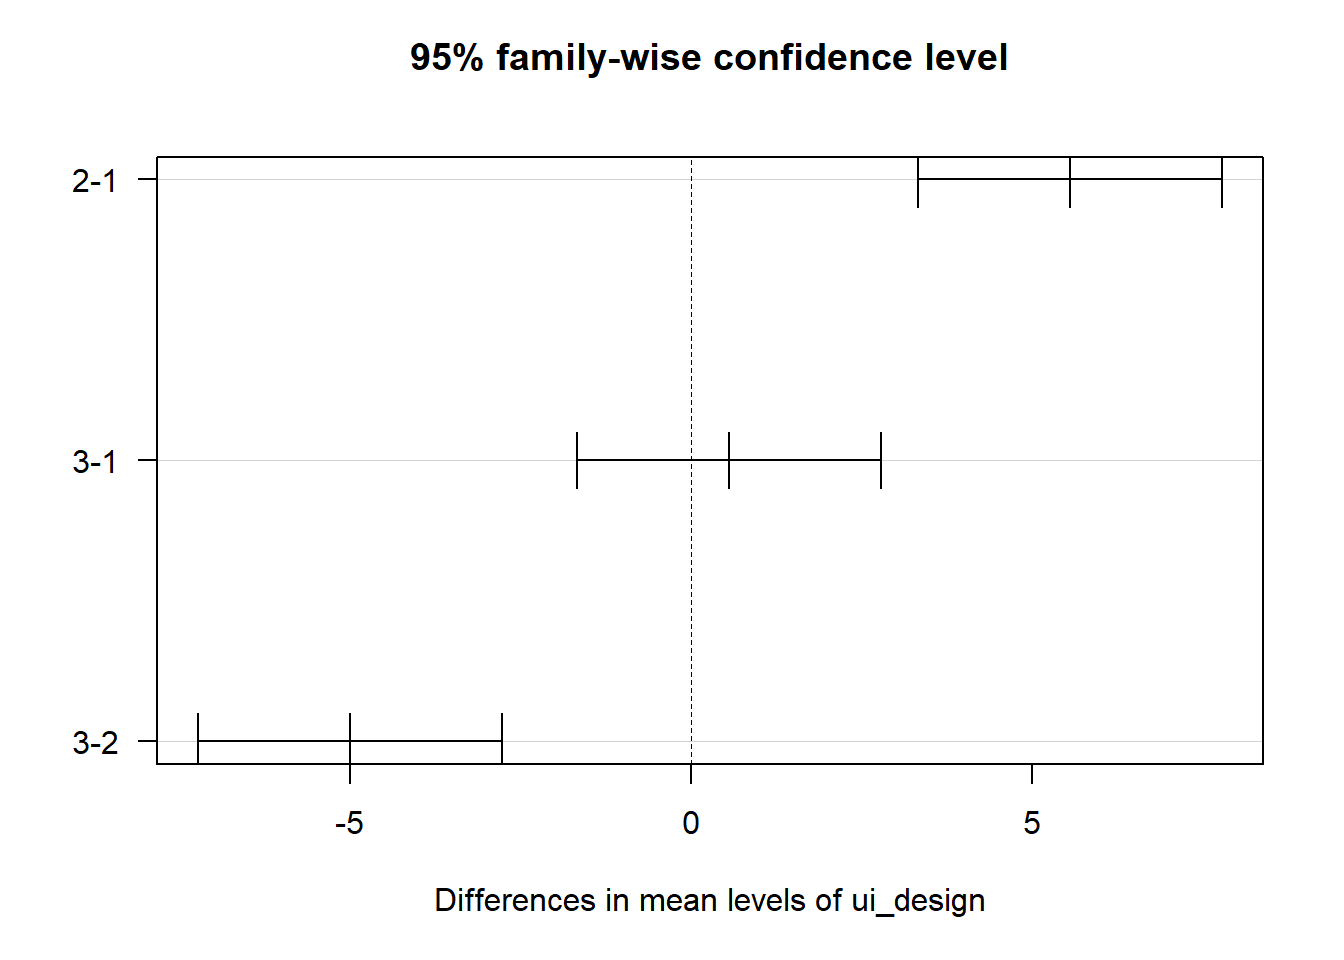
\includegraphics{ANOVA_files/figure-pdf/unnamed-chunk-10-1.pdf}

\begin{Shaded}
\begin{Highlighting}[]
\CommentTok{\# Creating a plot to visualize group means with confidence intervals}
\FunctionTok{ggplot}\NormalTok{(data, }\FunctionTok{aes}\NormalTok{(}\AttributeTok{x =}\NormalTok{ ui\_design, }\AttributeTok{y =}\NormalTok{ time\_spent)) }\SpecialCharTok{+}
  \FunctionTok{stat\_summary}\NormalTok{(}\AttributeTok{fun.data =}\NormalTok{ mean\_cl\_normal, }\AttributeTok{geom =} \StringTok{"errorbar"}\NormalTok{, }\AttributeTok{width =} \FloatTok{0.2}\NormalTok{) }\SpecialCharTok{+}
  \FunctionTok{stat\_summary}\NormalTok{(}\AttributeTok{fun =}\NormalTok{ mean, }\AttributeTok{geom =} \StringTok{"point"}\NormalTok{, }\AttributeTok{size =} \DecValTok{3}\NormalTok{) }\SpecialCharTok{+}
  \FunctionTok{labs}\NormalTok{(}\AttributeTok{title =} \StringTok{"Mean Time Spent on Website by UI Design"}\NormalTok{,}
       \AttributeTok{x =} \StringTok{"UI Design"}\NormalTok{,}
       \AttributeTok{y =} \StringTok{"Mean Time Spent (minutes)"}\NormalTok{) }\SpecialCharTok{+}
  \FunctionTok{theme\_minimal}\NormalTok{()}
\end{Highlighting}
\end{Shaded}

\begin{verbatim}
Warning: Computation failed in `stat_summary()`.
Caused by error in `fun.data()`:
! The package "Hmisc" is required.
\end{verbatim}

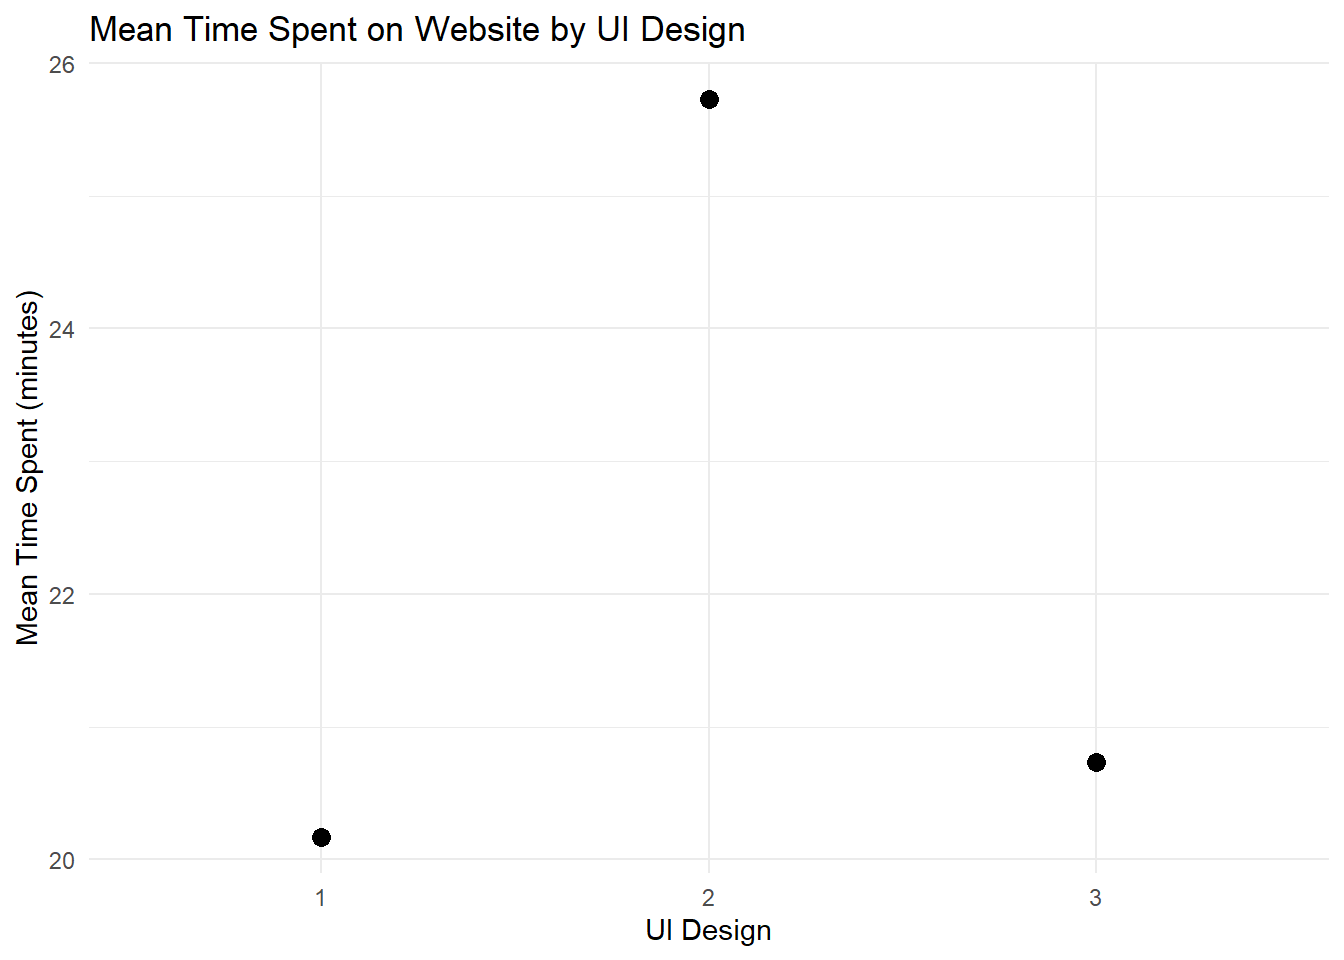
\includegraphics{ANOVA_files/figure-pdf/unnamed-chunk-10-2.pdf}

\section{Plotting the Results in
Stata}\label{plotting-the-results-in-stata}

\begin{Shaded}
\begin{Highlighting}[]
\NormalTok{* Plot }\FunctionTok{group} \KeywordTok{means}\NormalTok{ with confidence intervals}
\KeywordTok{means}\NormalTok{ time\_spent, }\BaseNTok{over}\NormalTok{(ui\_design) }\KeywordTok{ci}
\end{Highlighting}
\end{Shaded}

\section{Assumptions}\label{assumptions}

\begin{itemize}
\tightlist
\item
  \textbf{Independence}: Observations should be independent of each
  other.
\item
  \textbf{Normality}: The residuals of the model should be normally
  distributed.
\item
  \textbf{Homoscedasticity}: Variances across the groups should be
  equal.
\item
  \textbf{Random Sampling}: The data should be randomly sampled from the
  population.
\end{itemize}

These assumptions should be checked to ensure the validity of the ANOVA
results.

\section{Syntax Comparison: R vs
Stata}\label{syntax-comparison-r-vs-stata}

This table summarizes the main differences between R and Stata in terms
of syntax for performing ANOVA analyses.

\begin{longtable}[]{@{}
  >{\raggedright\arraybackslash}p{(\columnwidth - 4\tabcolsep) * \real{0.3097}}
  >{\raggedright\arraybackslash}p{(\columnwidth - 4\tabcolsep) * \real{0.3548}}
  >{\raggedright\arraybackslash}p{(\columnwidth - 4\tabcolsep) * \real{0.3355}}@{}}
\toprule\noalign{}
\begin{minipage}[b]{\linewidth}\raggedright
Task
\end{minipage} & \begin{minipage}[b]{\linewidth}\raggedright
R Command
\end{minipage} & \begin{minipage}[b]{\linewidth}\raggedright
Stata Command
\end{minipage} \\
\midrule\noalign{}
\endhead
\bottomrule\noalign{}
\endlastfoot
Simulating Data & \texttt{rnorm()} for simulating normal distribution &
\texttt{rnormal()} for simulating normal distribution \\
Setting Seed for Reproducibility & \texttt{set.seed(123)} &
\texttt{set\ seed\ 123} \\
Creating a Factor Variable & \texttt{factor()} & \texttt{gen\ variable}
and \texttt{egen\ group} \\
Visualizing Descriptives & \texttt{ggplot()} with
\texttt{geom\_boxplot()} & \texttt{graph\ box} \\
Running ANOVA & \texttt{aov()} and \texttt{summary()} &
\texttt{anova} \\
Post-hoc Testing & \texttt{TukeyHSD()} & \texttt{oneway} with
\texttt{bonferroni} option \\
Plotting Group Means with Confidence Intervals & \texttt{ggplot()} with
\texttt{stat\_summary()} & \texttt{means} with \texttt{ci} option \\
\end{longtable}

\bookmarksetup{startatroot}

\chapter{Linear Regression}\label{linear-regression}

\section{Introduction}\label{introduction-2}

This chapter covers how to perform linear regression to study the
relationship between variables. We'll use an example dataset that
simulates the relationship between study time and performance on an
online learning platform.

\section{Example Question}\label{example-question-1}

\textbf{How does the amount of time spent on an e-learning platform (in
hours) affect the test scores of users?}

\section{Dataset Simulation in R}\label{dataset-simulation-in-r}

\begin{Shaded}
\begin{Highlighting}[]
\CommentTok{\# Load necessary package}
\FunctionTok{set.seed}\NormalTok{(}\DecValTok{123}\NormalTok{)}

\CommentTok{\# Simulate data}
\NormalTok{n }\OtherTok{\textless{}{-}} \DecValTok{100}
\NormalTok{study\_time }\OtherTok{\textless{}{-}} \FunctionTok{rnorm}\NormalTok{(n, }\AttributeTok{mean =} \DecValTok{10}\NormalTok{, }\AttributeTok{sd =} \DecValTok{2}\NormalTok{)  }\CommentTok{\# Average 10 hours}
\NormalTok{test\_score }\OtherTok{\textless{}{-}} \DecValTok{50} \SpecialCharTok{+} \DecValTok{5} \SpecialCharTok{*}\NormalTok{ study\_time }\SpecialCharTok{+} \FunctionTok{rnorm}\NormalTok{(n, }\AttributeTok{mean =} \DecValTok{0}\NormalTok{, }\AttributeTok{sd =} \DecValTok{5}\NormalTok{)  }\CommentTok{\# Linear relationship with some noise}

\CommentTok{\# Create a data frame}
\NormalTok{data }\OtherTok{\textless{}{-}} \FunctionTok{data.frame}\NormalTok{(study\_time, test\_score)}

\CommentTok{\# View the first few rows}
\FunctionTok{head}\NormalTok{(data)}
\end{Highlighting}
\end{Shaded}

\section{Dataset Simulation in Stata}\label{dataset-simulation-in-stata}

\begin{Shaded}
\begin{Highlighting}[]
\NormalTok{* Set }\DecValTok{seed} \KeywordTok{for}\NormalTok{ reproducibility}
\KeywordTok{set} \DecValTok{seed}\NormalTok{ 123}

\NormalTok{* Simulate }\KeywordTok{data}
\KeywordTok{set} \KeywordTok{obs}\NormalTok{ 100}
\KeywordTok{gen}\NormalTok{ study\_time = rnormal(10, 2)}
\KeywordTok{gen}\NormalTok{ test\_score = 50 + 5 * study\_time + rnormal(0, 5)}

\NormalTok{* View the first few }\BaseNTok{rows}
\OtherTok{list} \KeywordTok{in}\NormalTok{ 1/10}
\end{Highlighting}
\end{Shaded}

\section{Performing Linear
Regression}\label{performing-linear-regression}

\subsection{R}\label{r-1}

\begin{Shaded}
\begin{Highlighting}[]
\CommentTok{\# Fit the linear regression model}
\NormalTok{model }\OtherTok{\textless{}{-}} \FunctionTok{lm}\NormalTok{(test\_score }\SpecialCharTok{\textasciitilde{}}\NormalTok{ study\_time, }\AttributeTok{data =}\NormalTok{ data)}

\CommentTok{\# View the summary}
\FunctionTok{summary}\NormalTok{(model)}
\end{Highlighting}
\end{Shaded}

\subsection{Stata}\label{stata-1}

\begin{Shaded}
\begin{Highlighting}[]
\NormalTok{* Fit the linear regression }\KeywordTok{model}
\KeywordTok{regress}\NormalTok{ test\_score study\_time}
\end{Highlighting}
\end{Shaded}

\section{Assumptions}\label{assumptions-1}

\begin{itemize}
\tightlist
\item
  \textbf{Linearity}: The relationship between the independent and
  dependent variable should be linear.
\item
  \textbf{Independence}: Observations should be independent of each
  other.
\item
  \textbf{Homoscedasticity}: The residuals should have constant variance
  at every level of the independent variable.
\item
  \textbf{Normality}: The residuals should be normally distributed.
\end{itemize}

\bookmarksetup{startatroot}

\chapter{Multilevel Regression}\label{multilevel-regression}

\section{Introduction}\label{introduction-3}

This chapter covers multilevel regression, where data is nested. We will
explore how user satisfaction with a mobile app is affected by time
spent on the app, considering that users are nested within different age
groups.

\section{Example Question}\label{example-question-2}

\textbf{Does time spent on a mobile app influence user satisfaction, and
does this effect differ across age groups?}

\section{Dataset Simulation in R}\label{dataset-simulation-in-r-1}

\begin{Shaded}
\begin{Highlighting}[]
\CommentTok{\# Load necessary package}
\FunctionTok{set.seed}\NormalTok{(}\DecValTok{123}\NormalTok{)}

\CommentTok{\# Simulate data}
\NormalTok{n\_groups }\OtherTok{\textless{}{-}} \DecValTok{5}  \CommentTok{\# Number of age groups}
\NormalTok{n\_per\_group }\OtherTok{\textless{}{-}} \DecValTok{50}  \CommentTok{\# Number of users per group}

\NormalTok{age\_group }\OtherTok{\textless{}{-}} \FunctionTok{factor}\NormalTok{(}\FunctionTok{rep}\NormalTok{(}\DecValTok{1}\SpecialCharTok{:}\NormalTok{n\_groups, }\AttributeTok{each =}\NormalTok{ n\_per\_group))}
\NormalTok{time\_spent }\OtherTok{\textless{}{-}} \FunctionTok{rnorm}\NormalTok{(n\_groups }\SpecialCharTok{*}\NormalTok{ n\_per\_group, }\AttributeTok{mean =} \DecValTok{30}\NormalTok{, }\AttributeTok{sd =} \DecValTok{10}\NormalTok{)}
\NormalTok{satisfaction }\OtherTok{\textless{}{-}} \DecValTok{3} \SpecialCharTok{+} \FloatTok{0.2} \SpecialCharTok{*}\NormalTok{ time\_spent }\SpecialCharTok{+} \FunctionTok{as.numeric}\NormalTok{(age\_group) }\SpecialCharTok{+} \FunctionTok{rnorm}\NormalTok{(n\_groups }\SpecialCharTok{*}\NormalTok{ n\_per\_group, }\AttributeTok{sd =} \DecValTok{2}\NormalTok{)}

\CommentTok{\# Create a data frame}
\NormalTok{data }\OtherTok{\textless{}{-}} \FunctionTok{data.frame}\NormalTok{(age\_group, time\_spent, satisfaction)}

\CommentTok{\# View the first few rows}
\FunctionTok{head}\NormalTok{(data)}
\end{Highlighting}
\end{Shaded}

\section{Dataset Simulation in
Stata}\label{dataset-simulation-in-stata-1}

\begin{Shaded}
\begin{Highlighting}[]
\NormalTok{* Set }\DecValTok{seed} \KeywordTok{for}\NormalTok{ reproducibility}
\KeywordTok{set} \DecValTok{seed}\NormalTok{ 123}

\NormalTok{* Simulate }\KeywordTok{data}
\KeywordTok{set} \KeywordTok{obs}\NormalTok{ 250}
\KeywordTok{gen} \FunctionTok{group}\NormalTok{ = }\FunctionTok{ceil}\NormalTok{(}\DataTypeTok{\_n}\NormalTok{/50)  }\CommentTok{// Age group}
\KeywordTok{gen}\NormalTok{ time\_spent = rnormal(30, 10)}
\KeywordTok{gen}\NormalTok{ satisfaction = 3 + 0.2 * time\_spent + }\FunctionTok{group}\NormalTok{ + rnormal(0, 2)}

\NormalTok{* Convert }\FunctionTok{group}\NormalTok{ to a }\KeywordTok{factor}
\KeywordTok{egen}\NormalTok{ group\_factor = }\FunctionTok{group}\NormalTok{(}\FunctionTok{group}\NormalTok{)}

\NormalTok{* View the first few }\BaseNTok{rows}
\OtherTok{list} \KeywordTok{in}\NormalTok{ 1/10}
\end{Highlighting}
\end{Shaded}

\section{Performing Multilevel
Regression}\label{performing-multilevel-regression}

\subsection{R}\label{r-2}

\begin{Shaded}
\begin{Highlighting}[]
\CommentTok{\# Load necessary package}
\FunctionTok{library}\NormalTok{(lme4)}

\CommentTok{\# Fit the multilevel model}
\NormalTok{model }\OtherTok{\textless{}{-}} \FunctionTok{lmer}\NormalTok{(satisfaction }\SpecialCharTok{\textasciitilde{}}\NormalTok{ time\_spent }\SpecialCharTok{+}\NormalTok{ (}\DecValTok{1} \SpecialCharTok{|}\NormalTok{ age\_group), }\AttributeTok{data =}\NormalTok{ data)}

\CommentTok{\# View the summary}
\FunctionTok{summary}\NormalTok{(model)}
\end{Highlighting}
\end{Shaded}

\subsection{Stata}\label{stata-2}

\begin{Shaded}
\begin{Highlighting}[]
\NormalTok{* Fit the multilevel }\KeywordTok{model}
\NormalTok{mixed satisfaction time\_spent || }\FunctionTok{group}\NormalTok{:}
\end{Highlighting}
\end{Shaded}

\section{Assumptions}\label{assumptions-2}

\begin{itemize}
\tightlist
\item
  \textbf{Normality of residuals}: The residuals at each level of the
  model should be normally distributed.
\item
  \textbf{Linearity}: The relationship between predictors and the
  outcome should be linear at each level of the model.
\item
  \textbf{Independence}: Observations within each group should be
  independent.
\item
  \textbf{Homoscedasticity}: The variance of residuals should be
  consistent across all levels of the hierarchy.
\end{itemize}

\bookmarksetup{startatroot}

\chapter{Logistic Regression}\label{logistic-regression}

\section{Introduction}\label{introduction-4}

This chapter covers logistic regression, which is used when the outcome
variable is binary. We will use an example dataset to investigate
whether the frequency of technical support contact predicts whether a
user continues to use a software product.

\section{Example Question}\label{example-question-3}

\textbf{Does the frequency of contacting technical support predict
whether a user will continue using a software product?}

\section{Required Packages (R)}\label{required-packages-r-1}

\begin{Shaded}
\begin{Highlighting}[]
\CommentTok{\# Load the necessary packages }
\FunctionTok{library}\NormalTok{(tidyverse) }\CommentTok{\# used for data manipulation and visualization}
\end{Highlighting}
\end{Shaded}

\begin{verbatim}
-- Attaching core tidyverse packages ------------------------ tidyverse 2.0.0 --
v dplyr     1.1.4     v readr     2.1.5
v forcats   1.0.0     v stringr   1.5.1
v ggplot2   3.5.0     v tibble    3.2.1
v lubridate 1.9.3     v tidyr     1.3.1
v purrr     1.0.2     
-- Conflicts ------------------------------------------ tidyverse_conflicts() --
x dplyr::filter() masks stats::filter()
x dplyr::lag()    masks stats::lag()
i Use the conflicted package (<http://conflicted.r-lib.org/>) to force all conflicts to become errors
\end{verbatim}

\begin{Shaded}
\begin{Highlighting}[]
\FunctionTok{library}\NormalTok{(broom) }\CommentTok{\# for tidying the model output, making it easier to work with}
\FunctionTok{library}\NormalTok{(Statamarkdown) }\CommentTok{\# to run Stata commands in an R environment}
\end{Highlighting}
\end{Shaded}

\begin{verbatim}
Stata found at C:/Program Files/Stata18/StataBE-64.exe
The 'stata' engine is ready to use.
\end{verbatim}

\begin{Shaded}
\begin{Highlighting}[]
\CommentTok{\# Statamarkdown configuration}
\NormalTok{stataexe }\OtherTok{\textless{}{-}} \StringTok{"C:/Program Files/Stata18/StataBE{-}64.exe"} \CommentTok{\# Add your own path to the Stata executable here if you want to try this out}
\NormalTok{knitr}\SpecialCharTok{::}\NormalTok{opts\_chunk}\SpecialCharTok{$}\FunctionTok{set}\NormalTok{(}\AttributeTok{engine.path=}\FunctionTok{list}\NormalTok{(}\AttributeTok{stata=}\NormalTok{stataexe))}

\CommentTok{\# to install any missing packages go to the Terminal and run the command: install.packages("PACKAGE\_NAME")}
\end{Highlighting}
\end{Shaded}

\section{Simulating the Dataset in
R}\label{simulating-the-dataset-in-r-1}

\begin{Shaded}
\begin{Highlighting}[]
\CommentTok{\# Setting a seed for reproducibility}
\FunctionTok{set.seed}\NormalTok{(}\DecValTok{123}\NormalTok{)}

\CommentTok{\# Simulating data}
\NormalTok{n }\OtherTok{\textless{}{-}} \DecValTok{200}
\NormalTok{support\_contact }\OtherTok{\textless{}{-}} \FunctionTok{rpois}\NormalTok{(n, }\AttributeTok{lambda =} \DecValTok{2}\NormalTok{)  }\CommentTok{\# Number of contacts with support}
\NormalTok{continued\_use }\OtherTok{\textless{}{-}} \FunctionTok{rbinom}\NormalTok{(n, }\AttributeTok{size =} \DecValTok{1}\NormalTok{, }\AttributeTok{prob =} \DecValTok{1} \SpecialCharTok{/}\NormalTok{ (}\DecValTok{1} \SpecialCharTok{+} \FunctionTok{exp}\NormalTok{(}\SpecialCharTok{{-}}\NormalTok{(}\SpecialCharTok{{-}}\DecValTok{1} \SpecialCharTok{+} \FloatTok{0.5} \SpecialCharTok{*}\NormalTok{ support\_contact))))}

\CommentTok{\# Creating a data frame}
\NormalTok{data }\OtherTok{\textless{}{-}} \FunctionTok{data.frame}\NormalTok{(support\_contact, continued\_use)}

\CommentTok{\# Viewing the first few rows of the dataset}
\FunctionTok{head}\NormalTok{(data)}
\end{Highlighting}
\end{Shaded}

\begin{verbatim}
  support_contact continued_use
1               1             0
2               3             0
3               2             1
4               4             1
5               4             1
6               0             1
\end{verbatim}

\section{Simulating the Dataset in
Stata}\label{simulating-the-dataset-in-stata-1}

\begin{Shaded}
\begin{Highlighting}[]
\NormalTok{* Set }\DecValTok{seed} \KeywordTok{for}\NormalTok{ reproducibility}
\KeywordTok{set} \DecValTok{seed}\NormalTok{ 123}

\NormalTok{* Simulate }\KeywordTok{data}
\KeywordTok{set} \KeywordTok{obs}\NormalTok{ 200}
\KeywordTok{gen}\NormalTok{ support\_contact = rpoisson(2)}
\KeywordTok{gen}\NormalTok{ continued\_use = rbinomial(1, 1 / (1 + }\FunctionTok{exp}\NormalTok{({-}({-}1 + 0.5 * support\_contact))))}

\NormalTok{* Save to }\KeywordTok{data}\NormalTok{ file}
\KeywordTok{save}\NormalTok{ logreg\_data.dta}

\NormalTok{* View the first few }\BaseNTok{rows}
\OtherTok{list} \KeywordTok{in}\NormalTok{ 1/10}
\end{Highlighting}
\end{Shaded}

\begin{verbatim}
Number of observations (_N) was 0, now 200.



file logreg_data.dta already exists
r(602);

r(602);
\end{verbatim}

\section{Visualizing the Descriptives in
R}\label{visualizing-the-descriptives-in-r-1}

\begin{Shaded}
\begin{Highlighting}[]
\CommentTok{\# Plotting the distribution of support contacts for users who continued vs those who didn\textquotesingle{}t}
\FunctionTok{ggplot}\NormalTok{(data, }\FunctionTok{aes}\NormalTok{(}\AttributeTok{x =} \FunctionTok{factor}\NormalTok{(continued\_use), }\AttributeTok{y =}\NormalTok{ support\_contact)) }\SpecialCharTok{+}
  \FunctionTok{geom\_boxplot}\NormalTok{() }\SpecialCharTok{+}
  \FunctionTok{labs}\NormalTok{(}\AttributeTok{title =} \StringTok{"Support Contacts vs Continued Use"}\NormalTok{,}
       \AttributeTok{x =} \StringTok{"Continued Use (0 = No, 1 = Yes)"}\NormalTok{,}
       \AttributeTok{y =} \StringTok{"Number of Support Contacts"}\NormalTok{)}
\end{Highlighting}
\end{Shaded}

\includegraphics{log_regression_files/figure-pdf/unnamed-chunk-4-1.pdf}

\section{Visualizing the Descriptives in
Stata}\label{visualizing-the-descriptives-in-stata-1}

\begin{Shaded}
\begin{Highlighting}[]
\NormalTok{* NO NEED TO LOAD DATA AGAIN If USING }\KeywordTok{STATA}
\KeywordTok{use}\NormalTok{ logreg\_data.dta}

\NormalTok{* Data summary}
\KeywordTok{summarize}
\end{Highlighting}
\end{Shaded}

\begin{verbatim}
    Variable |        Obs        Mean    Std. dev.       Min        Max
-------------+---------------------------------------------------------
support_co~t |        200       1.875    1.523476          0          8
continued_~e |        200        .435    .4970011          0          1
\end{verbatim}

\begin{Shaded}
\begin{Highlighting}[]
\NormalTok{* Box plot }\KeywordTok{of}\NormalTok{ support contacts }\KeywordTok{by}\NormalTok{ continued }\KeywordTok{use}
\KeywordTok{graph}\NormalTok{ box support\_contact, }\BaseNTok{over}\NormalTok{(continued\_use) }\BaseNTok{title}\NormalTok{(}\StringTok{"Support Contacts vs Continued Use"}\NormalTok{) b1title(}\StringTok{"Continued Use"} \StringTok{"No = 0, Yes = 1"}\NormalTok{) }\BaseNTok{ytitle}\NormalTok{(}\StringTok{"Number of Support Contacts"}\NormalTok{)}
\end{Highlighting}
\end{Shaded}

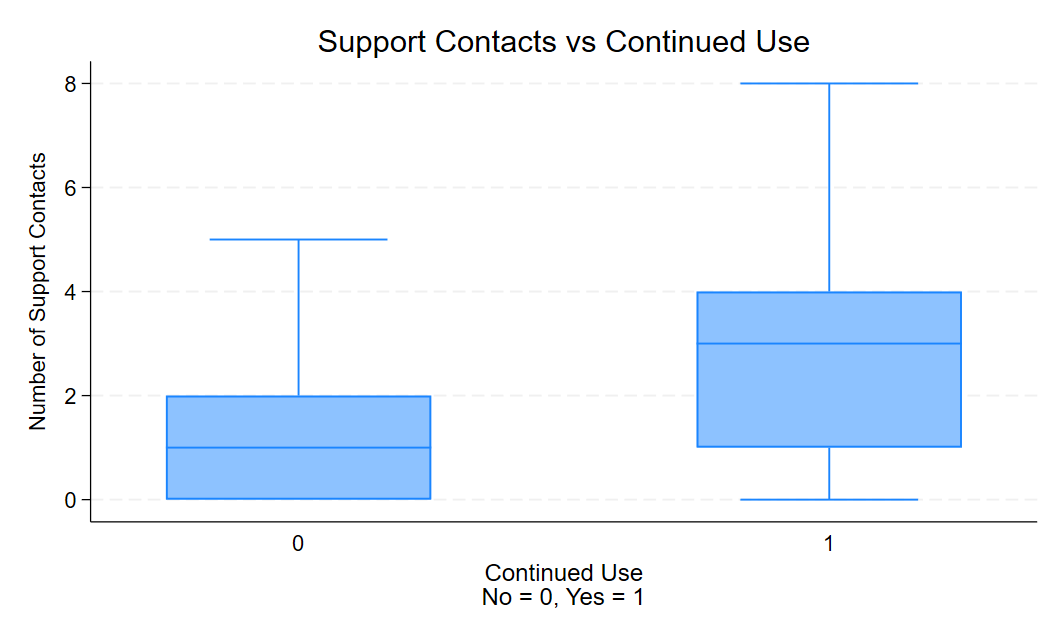
\includegraphics{images/log_regression_boxplot.png}

\section{Running the Logistic Regression in
R}\label{running-the-logistic-regression-in-r}

\begin{Shaded}
\begin{Highlighting}[]
\CommentTok{\# Fitting the logistic regression model}
\NormalTok{logistic\_model }\OtherTok{\textless{}{-}} \FunctionTok{glm}\NormalTok{(continued\_use }\SpecialCharTok{\textasciitilde{}}\NormalTok{ support\_contact, }\AttributeTok{data =}\NormalTok{ data, }\AttributeTok{family =} \StringTok{"binomial"}\NormalTok{)}

\CommentTok{\# Viewing the summary of the logistic regression model}
\FunctionTok{summary}\NormalTok{(logistic\_model)}
\end{Highlighting}
\end{Shaded}

\begin{verbatim}

Call:
glm(formula = continued_use ~ support_contact, family = "binomial", 
    data = data)

Coefficients:
                Estimate Std. Error z value Pr(>|z|)    
(Intercept)      -1.2023     0.3046  -3.947 7.90e-05 ***
support_contact   0.7398     0.1453   5.092 3.54e-07 ***
---
Signif. codes:  0 '***' 0.001 '**' 0.01 '*' 0.05 '.' 0.1 ' ' 1

(Dispersion parameter for binomial family taken to be 1)

    Null deviance: 274.83  on 199  degrees of freedom
Residual deviance: 240.15  on 198  degrees of freedom
AIC: 244.15

Number of Fisher Scoring iterations: 4
\end{verbatim}

\subsection{Output interpretation}\label{output-interpretation}

\begin{longtable}[]{@{}
  >{\raggedright\arraybackslash}p{(\columnwidth - 2\tabcolsep) * \real{0.2222}}
  >{\raggedright\arraybackslash}p{(\columnwidth - 2\tabcolsep) * \real{0.7778}}@{}}
\toprule\noalign{}
\begin{minipage}[b]{\linewidth}\raggedright
\textbf{Term}
\end{minipage} & \begin{minipage}[b]{\linewidth}\raggedright
\textbf{Description}
\end{minipage} \\
\midrule\noalign{}
\endhead
\bottomrule\noalign{}
\endlastfoot
\textbf{Coefficients} & Estimates of the regression coefficients. \\
\textbf{Std. Error} & Standard errors of the coefficients. \\
\textbf{z value} & The test statistic for each coefficient. \\
\textbf{Pr(\textgreater\textbar z\textbar)} & The p-value associated
with each coefficient, indicating whether it is statistically
significant. If the p-value is less than the significance level
(typically 0.05), we reject the null hypothesis that the coefficient is
equal to zero. \\
\end{longtable}

\section{Running the Logistic Regression in
Stata}\label{running-the-logistic-regression-in-stata}

\begin{Shaded}
\begin{Highlighting}[]
\NormalTok{* Loading }\KeywordTok{data}\NormalTok{ to make it work }\KeywordTok{in}\NormalTok{ R }\OtherTok{environment}\NormalTok{, YOU DO NOT NEED TO LOEAD THE DATA AGAIN IN }\KeywordTok{STATA}\NormalTok{ IF YOU ALREADY LOADED IT BEFORE!}
\KeywordTok{use}\NormalTok{ logreg\_data.dta}

\NormalTok{* Fit the }\KeywordTok{logistic}\NormalTok{ regression }\KeywordTok{model}
\KeywordTok{logit}\NormalTok{ continued\_use support\_contact}
\end{Highlighting}
\end{Shaded}

\begin{verbatim}
>  DATA AGAIN IN STATA IF YOU ALREADY LOADED IT BEFORE!


Iteration 0:  Log likelihood = -136.93464  
Iteration 1:  Log likelihood = -121.18683  
Iteration 2:  Log likelihood = -121.17434  
Iteration 3:  Log likelihood = -121.17434  

Logistic regression                                     Number of obs =    200
                                                        LR chi2(1)    =  31.52
                                                        Prob > chi2   = 0.0000
Log likelihood = -121.17434                             Pseudo R2     = 0.1151

------------------------------------------------------------------------------
continued_~e | Coefficient  Std. err.      z    P>|z|     [95% conf. interval]
-------------+----------------------------------------------------------------
support_co~t |    .589038   .1166492     5.05   0.000     .3604098    .8176661
       _cons |  -1.379241   .2688518    -5.13   0.000    -1.906181   -.8523008
------------------------------------------------------------------------------
\end{verbatim}

\subsection{Output description}\label{output-description}

\begin{longtable}[]{@{}
  >{\raggedright\arraybackslash}p{(\columnwidth - 2\tabcolsep) * \real{0.2222}}
  >{\raggedright\arraybackslash}p{(\columnwidth - 2\tabcolsep) * \real{0.7778}}@{}}
\toprule\noalign{}
\begin{minipage}[b]{\linewidth}\raggedright
\textbf{Term}
\end{minipage} & \begin{minipage}[b]{\linewidth}\raggedright
\textbf{Description}
\end{minipage} \\
\midrule\noalign{}
\endhead
\bottomrule\noalign{}
\endlastfoot
\textbf{Coef.} & Estimates of the regression coefficients. \\
\textbf{Std. Err.} & Standard errors of the coefficients. \\
\textbf{z} & The test statistic for each coefficient. \\
\textbf{P\textgreater\textbar z\textbar{}} & The p-value associated with
each coefficient, indicating whether it is statistically significant. If
the p-value is less than the significance level (typically 0.05), we
reject the null hypothesis that the coefficient is equal to zero. \\
\end{longtable}

\section{Plotting the Results in R}\label{plotting-the-results-in-r-1}

\begin{Shaded}
\begin{Highlighting}[]
\CommentTok{\# Plotting the logistic regression curve}
\FunctionTok{ggplot}\NormalTok{(data, }\FunctionTok{aes}\NormalTok{(}\AttributeTok{x =}\NormalTok{ support\_contact, }\AttributeTok{y =}\NormalTok{ continued\_use)) }\SpecialCharTok{+}
  \FunctionTok{geom\_point}\NormalTok{(}\AttributeTok{alpha =} \FloatTok{0.5}\NormalTok{) }\SpecialCharTok{+}
  \FunctionTok{geom\_smooth}\NormalTok{(}\AttributeTok{method =} \StringTok{"glm"}\NormalTok{, }\AttributeTok{method.args =} \FunctionTok{list}\NormalTok{(}\AttributeTok{family =} \StringTok{"binomial"}\NormalTok{), }\AttributeTok{se =} \ConstantTok{FALSE}\NormalTok{) }\SpecialCharTok{+}
  \FunctionTok{labs}\NormalTok{(}\AttributeTok{title =} \StringTok{"Logistic Regression: Probability of Continued Use"}\NormalTok{,}
       \AttributeTok{x =} \StringTok{"Number of Support Contacts"}\NormalTok{,}
       \AttributeTok{y =} \StringTok{"Probability of Continued Use"}\NormalTok{) }\SpecialCharTok{+}
  \FunctionTok{theme\_minimal}\NormalTok{()}
\end{Highlighting}
\end{Shaded}

\begin{verbatim}
`geom_smooth()` using formula = 'y ~ x'
\end{verbatim}

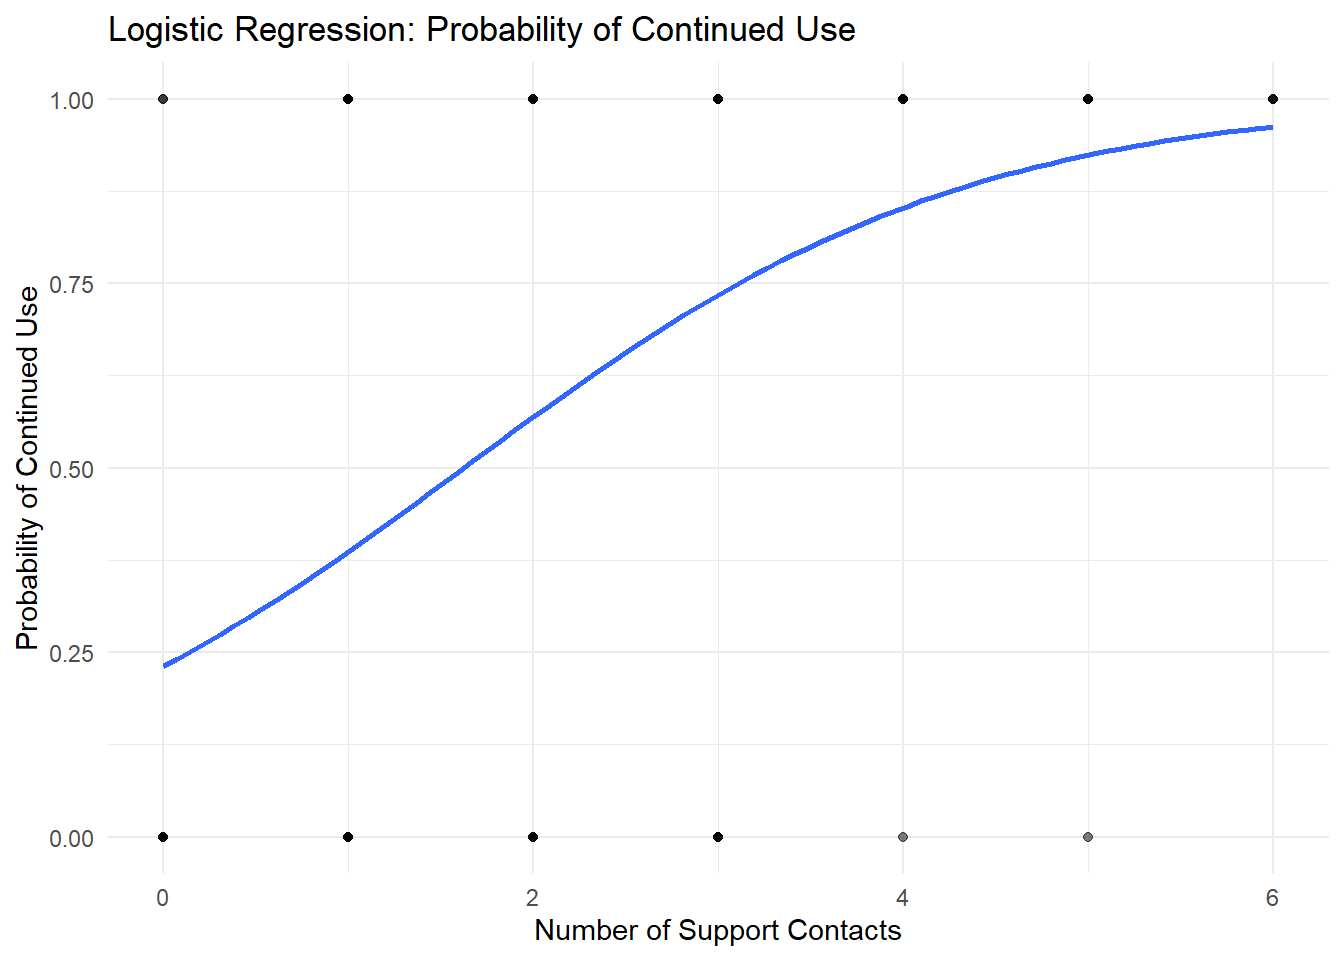
\includegraphics{log_regression_files/figure-pdf/unnamed-chunk-9-1.pdf}

\section{Plotting the Results in
Stata}\label{plotting-the-results-in-stata-1}

\begin{Shaded}
\begin{Highlighting}[]
\NormalTok{* Create }\KeywordTok{logistic}\NormalTok{ regression plot }

\CommentTok{/* Generate the predicted probabilities}
\CommentTok{This command generates the predicted probabilities from the logistic regression model and stores them in a new variable called \textquotesingle{}prob\textquotesingle{}.*/}
  
\KeywordTok{predict} \KeywordTok{prob}\NormalTok{, pr}

\CommentTok{/* Sort the data by the predictor variable. Sorting the data by \textquotesingle{}support\_contact\textquotesingle{} ensures that the line plot of predicted probabilities will be smooth and correctly ordered.*/}
  
\KeywordTok{sort}\NormalTok{ support\_contact}

\CommentTok{/* Plot the scatter plot with the logistic regression line This command creates a scatter plot of \textquotesingle{}continued\_use\textquotesingle{} against \textquotesingle{}support\_contact\textquotesingle{} and overlays it with a line plot of the predicted probabilities, which should form a sigmoidal curve.*/}

\KeywordTok{twoway}\NormalTok{ (}\KeywordTok{scatter}\NormalTok{ continued\_use support\_contact) (}\KeywordTok{line} \KeywordTok{prob}\NormalTok{ support\_contact)}
\end{Highlighting}
\end{Shaded}

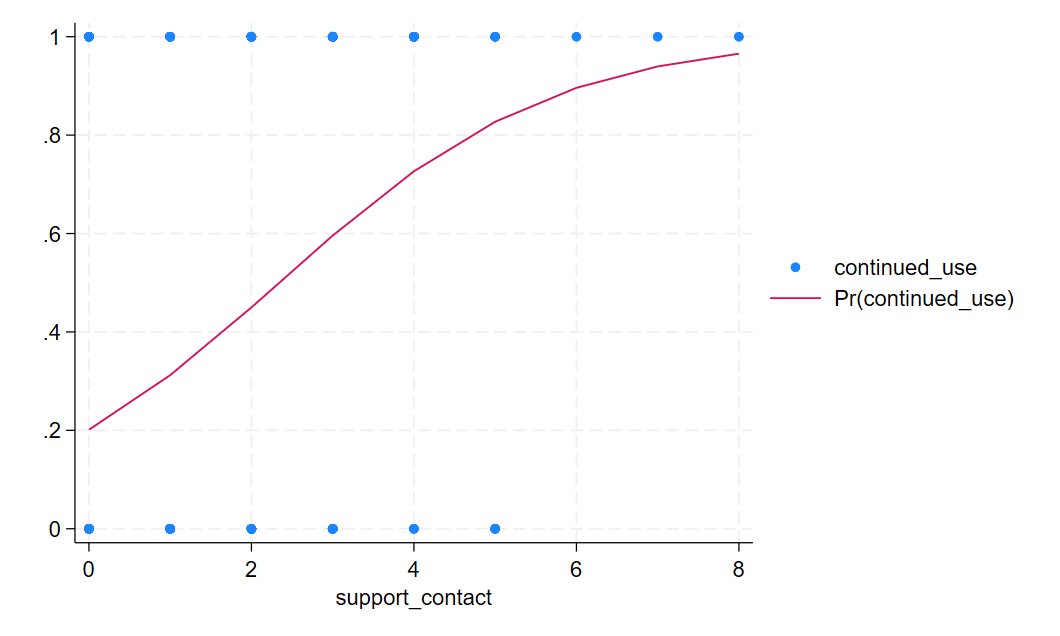
\includegraphics{images/log_regression_fitted.png}

\section{Assumptions}\label{assumptions-3}

\begin{longtable}[]{@{}
  >{\raggedright\arraybackslash}p{(\columnwidth - 2\tabcolsep) * \real{0.2636}}
  >{\raggedright\arraybackslash}p{(\columnwidth - 2\tabcolsep) * \real{0.7364}}@{}}
\toprule\noalign{}
\begin{minipage}[b]{\linewidth}\raggedright
\textbf{Assumption}
\end{minipage} & \begin{minipage}[b]{\linewidth}\raggedright
\textbf{Description}
\end{minipage} \\
\midrule\noalign{}
\endhead
\bottomrule\noalign{}
\endlastfoot
\textbf{Binary Outcome} & The dependent variable should be binary. \\
\textbf{Independence} & Observations should be independent of each
other. \\
\textbf{Linearity of logit} & The logit (log-odds) of the outcome should
be linearly related to the predictors. \\
\textbf{No multicollinearity} & The predictors should not be highly
correlated with each other. \\
\textbf{Large sample size} & Logistic regression typically requires a
large sample size to provide reliable estimates. \\
\end{longtable}

\section{R}\label{r-3}

\subsection{Binary oucome}\label{binary-oucome}

\begin{Shaded}
\begin{Highlighting}[]
\FunctionTok{table}\NormalTok{(data}\SpecialCharTok{$}\NormalTok{continued\_use)}
\end{Highlighting}
\end{Shaded}

\begin{verbatim}

  0   1 
 89 111 
\end{verbatim}

\subsection{Independence}\label{independence}

Verify that observations are independent. This is usually ensured by the
study design.

\subsubsection{Linearity of logit}\label{linearity-of-logit}

\begin{Shaded}
\begin{Highlighting}[]
\FunctionTok{library}\NormalTok{(car)}
\end{Highlighting}
\end{Shaded}

\begin{verbatim}
Loading required package: carData
\end{verbatim}

\begin{verbatim}

Attaching package: 'car'
\end{verbatim}

\begin{verbatim}
The following object is masked from 'package:dplyr':

    recode
\end{verbatim}

\begin{verbatim}
The following object is masked from 'package:purrr':

    some
\end{verbatim}

\begin{Shaded}
\begin{Highlighting}[]
\NormalTok{logit\_model }\OtherTok{\textless{}{-}} \FunctionTok{glm}\NormalTok{(continued\_use }\SpecialCharTok{\textasciitilde{}}\NormalTok{ support\_contact, }\AttributeTok{data =}\NormalTok{ data, }\AttributeTok{family =}\NormalTok{ binomial)}
\FunctionTok{crPlots}\NormalTok{(logit\_model)}
\end{Highlighting}
\end{Shaded}

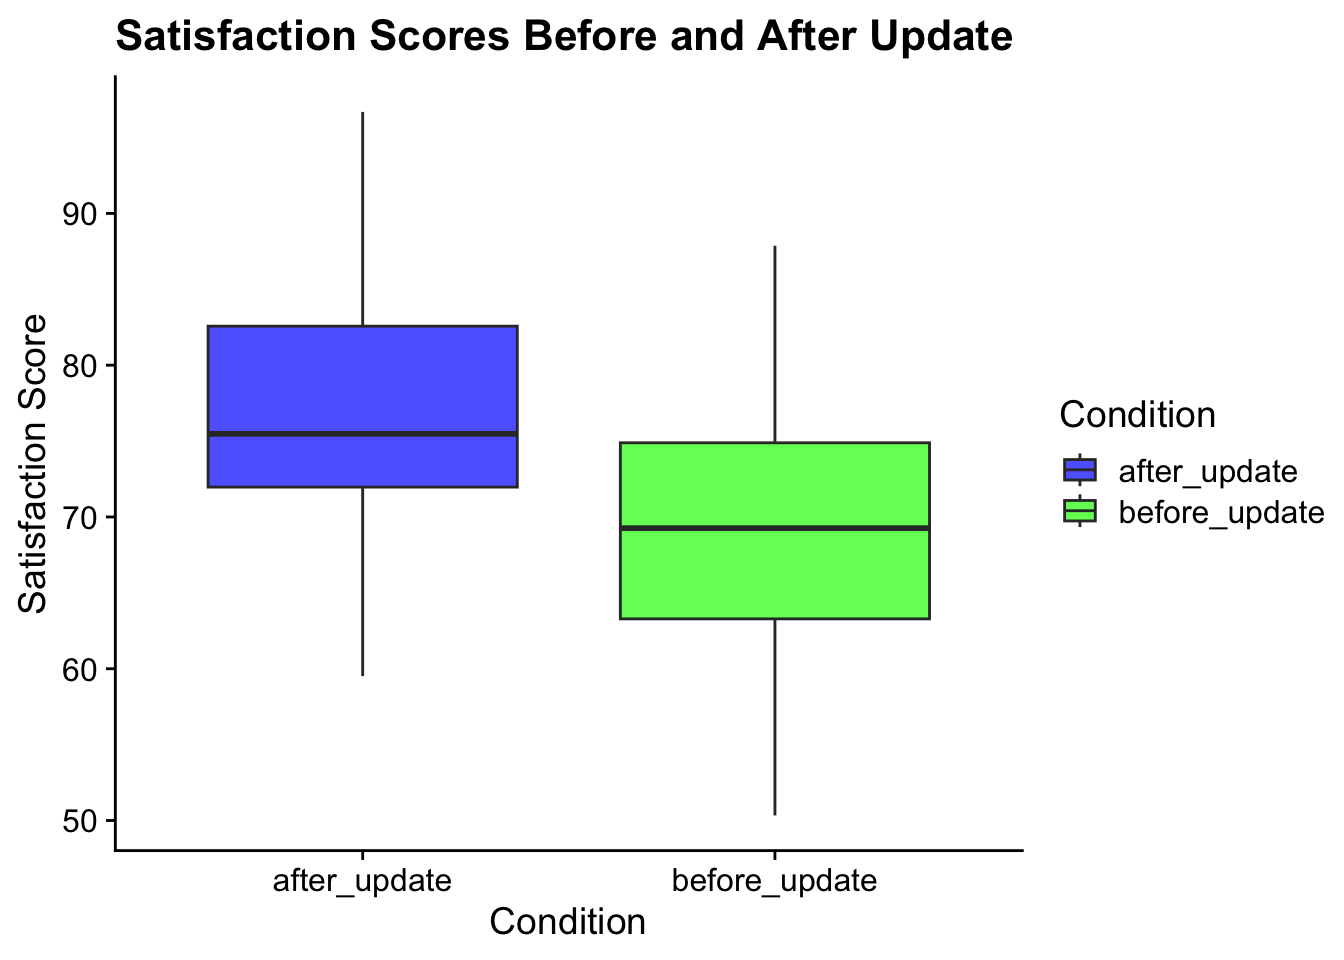
\includegraphics{log_regression_files/figure-pdf/unnamed-chunk-12-1.pdf}

\subsection{No Multicollinearity}\label{no-multicollinearity}

Note: The assumption of no multicollinearity is relevant only when you
have at least two predictors in your model. Multicollinearity occurs
when two or more predictors are highly correlated with each other, which
can make it difficult to determine the individual effect of each
predictor on the dependent variable.

Check for multicollinearity among predictors.

\begin{Shaded}
\begin{Highlighting}[]
\FunctionTok{vif}\NormalTok{(YOUR\_MODEL\_HER)}
\end{Highlighting}
\end{Shaded}

\begin{verbatim}
Error in eval(expr, envir, enclos): object 'YOUR_MODEL_HER' not found
\end{verbatim}

\subsection{Large sample size}\label{large-sample-size}

Ensure you have a sufficiently large sample size. A rule of thumb is at
least 10 events per predictor variable.

\section{Stata}\label{stata-3}

\subsection{Binary oucome}\label{binary-oucome-1}

\begin{Shaded}
\begin{Highlighting}[]
\KeywordTok{tabulate}\NormalTok{ continued\_use}
\end{Highlighting}
\end{Shaded}

\begin{verbatim}
no variables defined
r(111);

r(111);
\end{verbatim}

\subsection{Independence}\label{independence-1}

Verify that observations are independent. This is usually ensured by the
study design.

\subsection{Linearity of logit}\label{linearity-of-logit-1}

\begin{Shaded}
\begin{Highlighting}[]
\KeywordTok{gen}\NormalTok{ logit\_support\_contact = }\FunctionTok{log}\NormalTok{(support\_contact / (1 {-} support\_contact))}
\KeywordTok{scatter}\NormalTok{ logit\_support\_contact support\_contact}
\end{Highlighting}
\end{Shaded}

\begin{verbatim}
support_contact not found
r(111);

r(111);
\end{verbatim}

\subsection{No Multicollinearity}\label{no-multicollinearity-1}

\begin{Shaded}
\begin{Highlighting}[]
\KeywordTok{estat} \KeywordTok{vif}
\end{Highlighting}
\end{Shaded}

\begin{verbatim}
last estimates not found
r(301);

r(301);
\end{verbatim}

\subsection{Large sample size}\label{large-sample-size-1}

Ensure you have a sufficiently large sample size. A rule of thumb is at
least 10 events per predictor variable.

\section{Syntax Comparison: R vs
Stata}\label{syntax-comparison-r-vs-stata-1}

This table summarizes the main differences between R and Stata in terms
of syntax for performing Logistic Regression analysis.

\begin{longtable}[]{@{}
  >{\raggedright\arraybackslash}p{(\columnwidth - 4\tabcolsep) * \real{0.3151}}
  >{\raggedright\arraybackslash}p{(\columnwidth - 4\tabcolsep) * \real{0.3562}}
  >{\raggedright\arraybackslash}p{(\columnwidth - 4\tabcolsep) * \real{0.3288}}@{}}
\toprule\noalign{}
\begin{minipage}[b]{\linewidth}\raggedright
Task
\end{minipage} & \begin{minipage}[b]{\linewidth}\raggedright
R Command
\end{minipage} & \begin{minipage}[b]{\linewidth}\raggedright
Stata Command
\end{minipage} \\
\midrule\noalign{}
\endhead
\bottomrule\noalign{}
\endlastfoot
Simulating Data & \texttt{rpois()}, \texttt{rbinom()} &
\texttt{rpoisson()}, \texttt{rbinomial()} \\
Setting Seed for Reproducibility & \texttt{set.seed(123)} &
\texttt{set\ seed\ 123} \\
Visualizing Descriptives & \texttt{ggplot()} with
\texttt{geom\_boxplot()} & \texttt{graph\ box} \\
Running Logistic Regression & \texttt{glm()} with
\texttt{family\ =\ "binomial"} & \texttt{logit} \\
Plotting the Results & \texttt{ggplot()} with
\texttt{geom\_smooth(method\ =\ "glm",\ ...)} & \texttt{twoway\ scatter}
and \texttt{lfit} \\
\end{longtable}

\bookmarksetup{startatroot}

\chapter{Summary}\label{summary}

In summary, this book has no content whatsoever.

\begin{Shaded}
\begin{Highlighting}[]
\DecValTok{1} \SpecialCharTok{+} \DecValTok{1}
\end{Highlighting}
\end{Shaded}

\begin{verbatim}
[1] 2
\end{verbatim}

\bookmarksetup{startatroot}

\chapter*{References}\label{references}
\addcontentsline{toc}{chapter}{References}

\markboth{References}{References}

\phantomsection\label{refs}
\begin{CSLReferences}{0}{1}
\end{CSLReferences}



\end{document}
